








%\newcommand*{\ACM}{}%

\ifdefined\ACM

%\documentclass[sigplan,screen]{acmart}
\documentclass[manuscript,screen,review]{acmart}

\else
 \documentclass[12pt]{extarticle}
%\usepackage{libertine}
\usepackage{cuted}%\usepackage{widetext}
../synthesis/usepackage.tex
\usepackage{cancel}
\usepackage{tikz-3dplot}
\usepackage{subcaption}
\addbibresource{./sample.bib}

\fi
\usepackage{physics} 

\begin{document}
../synthesis/newcommands.tex
\title{ Coarse-Graining}
\author{David Ponarovsky}
\maketitle

% Constant depth fault tolerance construction.   
\newcommand*{\xb}{\mathbf{x}}

\ifdefined\SWEEPHEA
\else 
  \newcommand*{\SWEEPHEA}{}
  %\newcommand{\History}[1]{\mathbf{History}(#1)}
\newcommand{\History}[1]{H_{#1}}
  %\newcommand{\Time}[1]{\mathbf{Time}(#1)}
  \newcommand{\Time}[1]{T(#1)}
  \newcommand{\Excuse}[1]{\mathbf{Excuse}(#1)}
  \newcommand{\Excusei}[1]{\mathbf{Excuse}_{i}(#1)}
  \newcommand{\Size}[1]{\mathbf{Size}(#1)}
  \newcommand{\Span}[1]{\mathbf{Span}(#1)}
  \newcommand{\pre}[1]{\text{pre}(#1)}
  \newcommand{\poli}[1]{\text{pole}_{i}(#1)}
  \newcommand{\prei}[1]{\text{pre}_{i}(#1)}
  \newcommand{\predd}[1]{\text{pre}_{d+1}(#1)}
  \newcommand{\rotf}[2]{\theta_{#1 ,#2}}
  \newcommand*{\rotfs}{\rotf{v}{S^{\prime}}}
  \newcommand{\rotfv}[2]{\mathbf{\rotf{#1}{#2} }}
  \newcommand*{\rotfvs}{\mathbf{\rotfs{} }}
\fi

%\inb{\textbf{TODO:}}
%\begin{enumerate}
%
%
%  \item Enter that we care only about pauli errors somewhere. 
%  \item Rewrite the all outline. 
%
% % \item Define what is mean a finite chain. 
%
%  \item Mention that in 'applying the sweep rule on a chain', we refer to the application of the first stage of the sweep cycle. Namely, all the vertices work, yet we don't care about the dual base.
%  \item In all the claims about chains, set $x$ to note the default chain (instead $z$ which we keep to stabilizers) 
%  \item Change all the 'Pauli' to capital letter. 
%  \item Add after the definition of the computation DAG, that the order $J$ has to respect time order.  
%  %\item Enter the \textbf{Str} notation to the agreement claim. \Cref{claim:agreement}. 
%  \item Using \Cref{claim:polesmove} in \Cref{claim:shrinkslice} needs some work in the case that the slice contains multiple connected components. 
%\end{enumerate}

%\begin{abstract}
We suggest a new proof of quantum fault tolerance based on the alternative proofs of Toom's theorem \cite{Berman} (see also \cite{gacs2021newversiontoomsproof}). The fault tolerance construction is relative to the circuit model, subjected to local stochastic noise, where at each time unit only a constant depth of non-noisy classical computation is allowed. Our main error correction code is the $(d,d^{\prime})$-Toric code, namely qubits are set on the $d^{\prime}$-dimensional faces of the $d$-dimensional Toric. As byproducts of the study, we provide and prove the following:
  \begin{enumerate}
    \item  An explicit description of the sweep-rule —a generalization of Toom's rule for topological codes—for any dimension greater than two. In doing so, it answers affirmatively to the conjecture made by Kubica and Preskill \cite{Kubica_2019}.
    \item A fault tolerant construction in the circuit model that both uses the $(d,d^{\prime})$-Toric code and has a constant-depth correction cycle, where $d^{\prime}, d - d^{\prime} \ge 2$. Until now, the use of a topological code as the primary encoding and a constant-depth correction cycle were only achieved separately; this is the first work to achieve them simultaneously.
   
    \item A proof that the sweep-rule is an effective decoder against locally stochastic noise. Concurrently, denote by $n$ the side length of the $d$-dimensional Toric. If the noise rate is below a certain threshold, then an application of $\Theta(n^{2d +1})$ ideal sweep-cycle iterations erases the error with high probability. As far as we know, until now rigorous proofs for the sweep-rule were given only in the i.i.d setting \cite{Kubica_2019}. 

%    \item A novel fault tolerance that doesn't introduce an asymptotic depth overhead per Clifford gate. In particular, there is a threshold $p_{0} \in (0,1)$ such that for a noise rate $p < p_{0}$, and any $n$ large enough, the construction takes a circuit with total depth $\mu$ and a $\mathbf{T}$-depth $\mu_{\mathbf{T}}$, and results a circuit that simulates the given with probability: 
%      \begin{equation*}
%        \begin{split}
%          1 - \Theta ( \text{Poly(circuit's size)} ) p^{\Theta(n)}   
%        \end{split}
%      \end{equation*}
%      and has a depth $\Theta(\mu) + \Theta( \mu_{\mathbf{T}} n^{d+1} ) $. 
  \end{enumerate}
Specifically, all these results hold for the 4D-Toric code.
\end{abstract}

\tableofcontents
\newpage
%\section{Introduction}

\subsection{Background}

Fault-tolerant constructions take ideal quantum circuits and establish their logical equivalence such that they endure fault occurrences. Their efficiency is typically measured by the amount of additional resources – qubits, computation time, range connectivity, etc. – required by the resulting circuit, beyond the scope of theoretical discussion; those parameters translate into the machine complexity and energy cost required to run the circuits. Minimizing overheads brings quantum computing applications closer to the near future.

Since the introduction of the quantum threshold theorem \cite{aharonov1999faulttolerant}, which showed that quantum fault tolerance is in principle feasible, the main effort in subsequent work has focused on reducing the additional qubit overhead. A line of work has led to a constant-factor overhead in qubits, first in the instant-classical computation model \cite{gottesman2014faulttolerant}, then in the standard circuit model \cite{grospellier:tel-03364419}, \cite{Fawzi_2018}, \cite{ nguyen2025quantumfaulttoleranceconstantspace}. Yet, although the best qubit overhead was reached, the depth overhead was only slightly improved from poly-logarithmic to 'tilde'-logarithmic \cite{ nguyen2025quantumfaulttoleranceconstantspace}. In fact, it seems that the same means that are used to reduce the qubit overhead are the ones that challenge reducing the depth overhead.    

A key concept for reducing qubit overhead is to encode qubits with a high-rate quantum LDPC code.  For those codes, except for the control-not, there are no known gates that can be realized in constant depth; furthermore, since the structure of the codes is relatively complicated – based on the skeletons of expander graphs - it seems hard to look for realizations of their logical operators. Without a constant-depth realization of logical operators, any construction that doesn't interfere with the order of the logical operations would admit a non constant-depth overhead. 

Contrary to high-rate LDPC codes, topological error codes have a geometrical image that is well understood and, as a result, a wide range of works suggest efficient realization of their logical operators. For example, consider the 3D-color code \cite{Bombín_2015}, fold-transversal gates on the surface code \cite{Breuckmann_2024}, and realization of the Clifford group on the 2D Toric \cite{guernut2024faulttolerantconstantdepthcliffordgates}.

Another branch of work, whose primary goal was to show that the embedding dimension of the computation can be reduced to 2D \cite{Balasubramanian_2026}, and more recently \cite{dünnweber2026quantummemoryautonomouscomputation}, uses topological codes as the main error correction code. Those constructions simplify the hardware realization; they suggest that quantum computers can be implemented by nearest-neighbor interactions automata - what is believed to be easier to develop. Yet, as in the threshold theorem \cite{aharonov1999faulttolerant}, and in contrast to the works that use high-rate LDPC codes, they rely on a hierarchical correction cycle whose execution time grows with system size. Hence, even though those directions have the potential to overcome the non-constant depth overhead per gate, it seems that the correction cycle imposes a barrier for them to come up with a constant factor in depth-overhead construction. 

\subsection{Stating Our Results}
%\paragraph{Fault Tolerance Using the 4D-Toric, Without Hierarchical Correction.}
In this work, we present a fault-tolerance construction that uses the $(d,d^{\prime})$-Toric code and has a constant-depth 'correction' cycle, for any $d^{\prime},d-d^{\prime} \ge 2$. In other words, the construction uses a relatively simple code - the 4D Toric code, yet doesn't incur the cost of a hierarchical correction cycle.

The computation model we consider is quantum circuits subject to \textit{local-stochastic noise}, where only qubits are subjected to the noise, while classical bits are non-noisy. Classical computation is allowed, and the classical depth matters. Namely, at each time unit, only a constant depth of classical computation can be done.  Local stochastic channel is defined to act such that the probability of any subset of locations $S$ (space-time coordinates), which is picked prior to the channel's action, being affected decays exponentially with the subset size. 
\begin{definition}[Local stochastic noise channel]
  Let $p\in(0,1)$. We say that the noise channel $\mathcal{N}_{\mathcal{E}}$ is \textit{local stochastic with rate $p$} if for every finite set of locations $S\subset \mathbb{N}\times \mathbb{N}$,
  \begin{equation*}
    \begin{split}
      \prbm{S\subset \operatorname{Loc}(\mathcal{E})}{\mathcal{E}\sim \mathcal{N}_{\mathcal{E}}}
      \le p^{|S|}.
    \end{split}
  \end{equation*}
\end{definition}

For circuits $\tilde{C}$ and $C$, we say that $\tilde{C}$ simulates $C$ with probability $p$ if, when one stops a noisy run of $\tilde{C}$ at a midpoint, one can, with probability $p$, recover by non-noisy operation an 'image' of a midpoint in the running of $C$, and if stopping at the last time point of $\tilde{C}$ enables recovery of the 'image' of $C$ at the end of its run. We state our main theorem as follows:
\begin{theorem*}[Informal version of \Cref{theorem:main}]
  There exists a constant $p_{0} \in (0,1)$ such that for any local stochastic noise channel $\mathcal{N}_{\mathcal{E}}$ with rate $p < p_{0}$, a quantum circuit $C$ with depth $\mu$ and width $w$, and a big enough integer $n$, there exists a 'logical equivalence' circuit $\tilde{C}$ with depth $\Theta(\mu n^{5})$ and width $\Theta((w + \mu) n^{8} \text{Polylog} (n) )$ that simulates $C$ with probability:
\begin{equation*}
  \begin{split}
    1 -   O \left( \text{poly}(w,\mu,n) \right)  p^{\Omega(n)} 
  \end{split}
\end{equation*}
Furthermore, $\tilde{C}$ has the following two properties:
\begin{enumerate}
  \item After a short initialization stage (at depth $\Theta( \text{Poly}(\log n))$), each of the qubits is encoded in the $n$-length 4D Toric code.
  \item An error correction cycle takes $O(1)$ depth, and the gates in each correction cycle don't depend on time. In particular, if $C$ is the identity circuit, then after the initialization stage, the layers in $\tilde{C}$ are the same constant-depth error reduction procedure.
\end{enumerate}
  \end{theorem*} 
As mentioned earlier, both code simplicity and error correction cycles at constant depth have already been achieved: the former as part of the quantum automation line of work, and the latter through the use of high-rate error correction codes. However, this is the first construction to achieve both simultaneously. %\Cref{fig:comparereresults} summarizes and compares the different works:


%\newcommand{\tcite}[1]{\hfill\cite{#1}}
%%\scalebox{0.8}{
%  \begin{table}[h]
%    %\centering
%    %\setlength{\tabcolsep}{4pt}
%    {
%      \footnotesize
%      \begin{tabular}{l p{4cm} p{3cm} p{2cm} p{3cm}}
%        \toprule
%        {\sc Works Line }  &   	\textsc{Error correction \newline code}  &   \textsc{Constant-depth \newline correction \newline cycle}   &   \textsc{Depth/qubit \newline overhead }  &  \textsc{Ref}    \\
%        \midrule
%        {\sc Concatenation }   & Concatenation of \newline fixed length code  & \ding{55}  & $f(x)$  & \cite{aharonov1999faulttolerant} \\
%        {\sc High-rate }       & Quantum expanders/ good QLDPC &  \ding{51}     & $f(x)$ &  \cite{grospellier:tel-03364419}, \cite{Fawzi_2018}, \cite{nguyen2025quantumfaulttoleranceconstantspace}  \\
%        {\sc Quantum Automata } & 2D-Toric code    & \ding{55}        & $f(x)$ &  \cite{Balasubramanian_2026}, \cite{dünnweber2026quantummemoryautonomouscomputation}  \\
%        {\sc Ours}             & 4D-Toric code    & \ding{51}                            & $f(x)$ & \\
%        \bottomrule
%      \end{tabular}
%
%    }
%    \caption{\label{fig:comapreresults} Comparing different types of works on fault-tolerance. }
%  \end{table}

%  \paragraph{Clifford-free Depth Overhead.}  An application that results from a slight modification of the main construction and its proof is a fault-tolerant construction that introduces a constant depth overhead per Clifford gate. We name that construction \textit{Clifford-free Depth Overhead}. \Cref{section:cliffordfree} describes the construction, proves external claims that are needed, and eventually elaborates on how to modify the proof of the main theorem to achieve the desired result.
%
%  \begin{theorem*}[Informal version of \Cref{theorem:cliffordfree}]
%    There exists a constant $ p_{0} \in (0,1) $ such that for any local stochastic noise channel $\mathcal{N}_{\mathcal{E}}$ with rate $ p < p_{0} $, and a Clifford+$\mathbf{T}$ quantum circuit $ C $ with depth $\mu$, $\mathbf{T}$-depth $\mu_{\mathbf{T}}$ and width $ w $, there exists a 'logical equivalence' circuit $\tilde{C}$, with depth $ \Theta(\mu) + \Theta( \mu_{\mathbf{T}} n^{5}) $ and width $\Theta((w + \mu) n^{8} \text{Polylog} (n) )$ that simulates $ C $ with probability:
%\begin{equation*}
%  \begin{split}
%    1 -   O \left( \text{poly}(w,\mu,n) \right)  p^{\Omega(n)} 
%  \end{split}
%\end{equation*}
%  \end{theorem*} 

  \paragraph{Sweep-rule in High Dimensions.} 
  The correction cycle in our construction consists of local operations done in parallel. Concurrently, any vertex of the Toric is thought of as a computation unit that has to decide on a correction to be applied over its local neighborhood. The specific procedure it runs is the sweep-rule, a generalization of Toom's rule invented by Kubica and Preskill \cite{Kubica_2019}. The sweep-rule can be sketched informally as follows: The vertex looks for a subset of bits to flip on its 'first quarter'\footnote{or the positive direction}, such that the flipping erases the syndrome that is seen on the 'first quarter' and all the bits to be flipped are supported on vertices that support the local syndrome. If there is such a subset of bits, then the vertex flips the bits. In \cite{Kubica_2019}, it is argued that for small dimensions, any vertex that sees only syndrome on its 'first quarter' has a subset of bits to be flipped that satisfy the sweep-rule requirement. Moreover, the authors conjectured that this is also true for higher dimensions. We prove their conjecture; furthermore, we give an explicit algorithm for finding the subset. We refer to the outline section for an elaborated discussion.
 

  \paragraph{Sweep-rule as Ideal Decoder Against Local Stochastic Noise.} 
A proof that the sweep-rule is an effective decoder against locally stochastic noise. Concurrently, denote by $n$ the side length of the $d$-dimensional Toric. If the noise rate is below a certain threshold, then an application of $\Theta(n^{2d +1})$ ideal sweep-cycle iterations erases the error with high probability. As far as we know, until now rigorous proofs for the sweep-rule were given only in the i.i.d setting \cite{Kubica_2019}. 


\subsection{Discussions, Applications, and Further Directions}
Our result can be understood as follow: when the qubit overhead is not a consideration, it means that the 4D Toric code is might be as good as the good quantum LDPC / Hyperproduct code. That translates to the two following applications: 
\begin{enumerate}
  \item New approach for quantum fault tolerance: Our proof is inherently different from prior works, describes in higher resolution the expected error, and might be used as a springboard for a constant depth overhead construction. %Furthermore, claims whose correctness follows from a constant depth overhead construction might be reconsidered in the lens of Clifford-free depth overhead. For example, in the context of \textbf{qPCP} with logarithmic soundness \cite{Anshu_2024}, we suggest that a realization of '$n$-bitwise OR' at logarithmic depth and constant $\mathbf{T}$-depth, combined with our Clifford-free construction, might give the '\textbf{qPCP} with logarithmic soundness' theorem.
    \item Memory/Storage components: Protecting a 4D Toric encoded state for an exponentially long time is achieved by performing the same operation at each time unit, suggesting that the 4D Toric code is a promising candidate for memory in the circuit model. Combined with the fact that the 4D Toric code also functions as memory in thermal noise models \cite{alicki2008thermalstabilitytopologicalqubit}, and given its relative simplicity, it appears to be a natural choice for real-world memory applications. We emphasize that an experimental usage of codes in four dimensions has already been demonstrated \cite{aasen2025topologicallyfaulttolerantquantumcomputer}, \cite{Berthusen_2024}, \cite{reichardt2024demonstrationquantumcomputationerror}.
\end{enumerate}






\section{Outline of the Proof}
In studying fault tolerance, the typical method is to first distinguish between configurations that can be tolerated and those that cannot. For example, in von Neumann-style proofs \cite{Neumann+1956+43+98}, it is common to track the number of flipped bits; if fewer than half are flipped, the logical states can be recovered. In the work of Aharonov and Ben-Or \cite{aharonov1999faulttolerant}, a logical bit at the $n$ level admits a logical error if at least a constant fraction of the $n-1$ level logical bits that compose it admit an error. In the work of \cite{grospellier:tel-03364419}, a tolerated configuration is one in which all encoded registers can be considered as distributed according to sufficiently weak local stochastic noise. The next step is to show that from a tolerated configuration, we move with high probability to another tolerated configuration. For our goals, each approach presents a challenge: The concatenation method, by definition, requires non-trivial depth computation at each step. Tracking the number of flipped bits fails almost immediately, as topological error correction codes have sublinear distance when a linear number of bits is expected to be flipped. And preserving the local stochastic noise distribution seems to heavily rely on the expansion properties \cite{grospellier:tel-03364419} of the underlying structure, where for topological codes, we expect to forge a 'spatial' dependence.


In  contrast, Berman and Simon provided a proof that, instead of tracking the dynamics, considers the entire run as a possible outcome, ruling out improbable runs only at the end \cite{Berman}. We outline their idea informally as follows: a logical bit is represented by $n \times n$ bits set on the vertices of the grid. In each correction cycle, the bits determine their value by taking the majority of their current value, and their north and east neighbors values, a rule known as Toom's rule. For simplicity, let's ignore the logical operations. Now, given a run, and in particular the set of space-time locations of faults, consider the following directed graph $\mathcal{H} \colonequals (V_{\mathcal{H}}, E_{\mathcal{H}})$ induced by it: 
\begin{enumerate}
  \item If at time $t$, the bit at vertex $v$ diverges relative to the ideal run, then add $(v,t)$ to the vertices. 
  \item If at time $t$, vertex $v$ 'leads' one of its neighbors $u$ to diverge, then connect $(v,t)$ and $(u,t+1)$ by an 'arrow'. 
  \item Connect any two vertices in $V_{\mathcal{H}}$, which are connected to a third by 'arrows', by a 'fork'. 
\end{enumerate}
Notice that the vertices of $\mathcal{H}$ with no incoming arrows correspond to faults; let's call them leaves. Thus, the probability of each running can be bounded by the number of leaves in the induced graph. Their key lemma states that a cluster of flipped bits with a 'perimeter' $s$, connected by arrows, induces a subgraph with at least $\Theta(s)$ leaves\footnote{ And number of edges $\le \Theta( \text{leaves} ) $.}. In other words, the probability of a connected component (by arrows) being flipped decays exponentially with its perimeter. 


The graph $\mathcal{H}$ was later named Toom's contours, a term that, to the best of our knowledge, was coined in \cite{swart2026peierlsboundstoomcontours}.
We chose to follow their approach. The rest of the section reviews the challenges that we encountered on the way to generalize it and the ideas to overcome them.


\paragraph{The Toric Code, the Sweep-Rule, and the Infinite Plane.}
%\label{subsection:toric}
The first issue was finding an analog for Toom's rule. We decided to adopt the sweep rule invented by Preskill and Kubica in \cite{Kubica_2019}, which they introduced as a local rule for any CSS code induced by a simplicial Toric, equipped with a notion of 'positive' and 'negative' directions (in their paper 'future' and 'past'). They also provided a rigorous proof that the iterative non-noisy applications of the sweep rule succeed in decoding faults that were sampled independently. For our purposes, we had to extend their proof for cubical Toric\footnote{The standard Toric codes.}. The main reason for this is that the alignment of the positive/negative directions with the axes direction of $\mathbb{R}^{d}$ space allows quantifying the 'perimeter' of error clusters. Yet, we are sure that our proof can be adjusted to support simplicial Toric complexes as well, and we leave it for further work.

%In the formal section, we define and prove the claims for Torices in any dimension greater than two, except for \Cref{claim:agreement}, which we proved only to dimension four. (Yet a numerical study hints that the claim might also be generalized; see \Cref{conj:agreement}.)


In complete contrast to typical works in topology, where global properties are studied and local characterization is left as general as possible, here we need notations to describe the local view of each vertex of the complex. We needed it for defining the sweep-rule action and stating claims about how it shrinks errors. That led us to the $\rotfvs{}$ notation defined in detail in \Cref{def:toric_complex}. In general, we denote by $S$ the generator set of the Toric, and for a subset of generators $S^{\prime} \subset S$, we define $\rotfvs{ }$ to be the face whose 'bottom-left' corner is the vertex $v$, and sides of the face correspond to edges on paths obtained by stepping through subsets of $S^{\prime}$ (for example, if $S^{\prime} = \{g_{1},g_{2},g_{3} \}$ then $\{g_{2}g_{1}v, g_{3}g_{2}g_{1}v\}$ is an edge of $\rotfvs{}$).  \Cref{fig:Toric} shows how the 2D-Toric complex is characterized via $\rotfvs{}$ notation.     \begin{figure}[h]

\begin{center}
    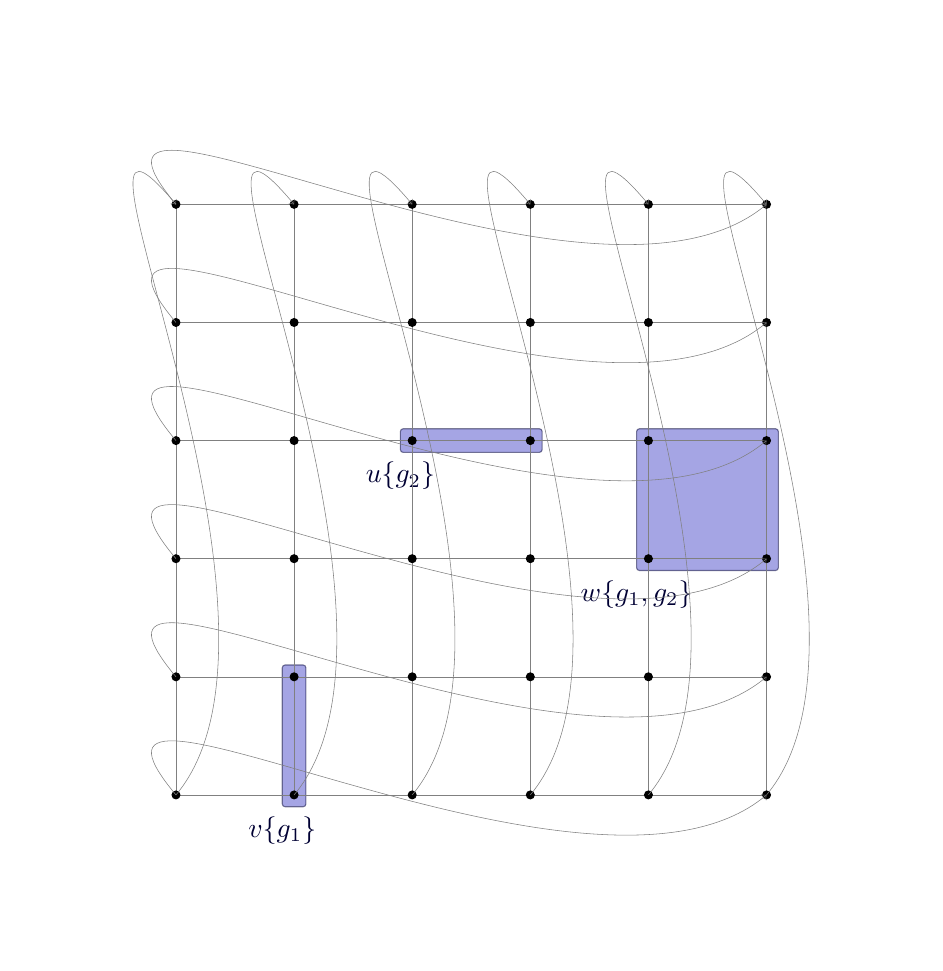
\begin{tikzpicture}[scale=1.5]


  \draw[blue!20!black,fill=blue!70!black!70,rounded corners=1, opacity=0.5]%shift={(0.15,0.15)}]
  (0.9,-0.1) node[below, opacity=1] {$\rotfv{v}{\{ g_{1}\} } $}
  rectangle (1.1,1.1);

  \draw[blue!20!black,fill=blue!70!black!70,rounded corners=1, opacity=0.5]%,shift={(0.15,0.15)}]
  (1.9,2.9) node[below, opacity=1] {$\rotfv{u}{\{ g_{2} \} }$} 
  rectangle (3.1,3.1);

  \draw[blue!20!black,fill=blue!70!black!70,rounded corners=1, opacity=0.5]%,shift={(0.15,0.15)}]
  (3.9,1.9) node[below, opacity=1] {$\rotfv{w}{\{g_{1}, g_{2} \} }$} 
  rectangle (5.1,3.1);

  \draw[step=1cm,gray,very thin] (0,0) grid (5,5);
  \foreach \x in {0,1,2,3,4,5}
  \foreach \y in {0,1,2,3,4,5}
  {
  \node[draw,circle,inner sep=1pt,fill] at (\x,\y) {};
}
\draw[gray,very thin,-> ]  (0,0) to [out=50, in=130] (0,5);
\draw[gray,very thin,-> ]  (1,0) to [out=50, in=130] (1,5);
\draw[gray,very thin,-> ]  (2,0) to [out=50, in=130] (2,5);
\draw[gray,very thin,-> ]  (3,0) to [out=50, in=130] (3,5);
\draw[gray,very thin,-> ]  (4,0) to [out=50, in=130] (4,5);
\draw[gray,very thin,-> ]  (5,0) to [out=50, in=130] (5,5);
\draw[gray,very thin,-> ]  (0,5) to [out=130, in=220] (5,5);
\draw[gray,very thin,-> ]  (0,4) to [out=130, in=220] (5,4);
\draw[gray,very thin,-> ]  (0,3) to [out=130, in=220] (5,3);
\draw[gray,very thin,-> ]  (0,2) to [out=130, in=220] (5,2);
\draw[gray,very thin,-> ]  (0,1) to [out=130, in=220] (5,1);
\draw[gray,very thin,-> ]  (0,0) to [out=130, in=220] (5,0);


\end{tikzpicture}
\end{center}
\caption{ Here we consider a 2D Toric complex. We name the set of generators $S= \{ g_{1},g_{2} \}$, where $g_{1}$ is the generator that sends us one step in the north direction, and $g_{2}$ sends us in the east direction. For vertices $v, u, w$, we mark in blue three faces that are rooted at them. }
\label{fig:Toric}
\end{figure}

 


The 4D-Toric code is defined as the binary assignment over the 2D-faces (plaquettes), where the $Z$-stabilizers (parity checks) are set on the edges, namely restrict the $Z$ product of the faces adjacent to each edge, and the $X$-stabilizers (phase checks) are set on the 4D-faces (hypercubes). Similarly, the $(d,d^{\prime})$-Toric code is defined by associating the $d^{\prime}$-dimensional faces of the $d$-dimensional Toric code with the qubits, while associating the $d^{\prime}\pm 1$-dimensional faces with the $X/Z$-stabilizers.


To present the sweep-rule, we need to have a definition of directions. For this section, we will be satisfied with the following hand-waving: For a vertex $v$, the bits and checks on the first 'quarter' of it (high-dimensional quarter) will be named the positive bits and checks of $v$.
\begin{definition}[Sweep Rule (Inforaml)]
  Let $z$ be a binary assignment on the Toric faces representing 'error'. The \textit{sweep rule decoding procedure} at a vertex $v$ is defined as follows:


Measure the positive checks of $v$ and denote the outcome by $\sigma$. Next, look for an assignment $\tilde{z}$ on the positive bits of $v$ such that the vertex support of $\tilde{z}$ is contained in the vertex support of $\sigma$ and that the positive checks of $v$ assign to $\tilde{z}$ the same syndrome as $\sigma$. If there is such, flip $\tilde{z}$.

\end{definition}
See \Cref{def:sweeprule} for the formal version. A full error correction cycle, or a sweep-cycle, consists of applying the sweep-rule to each vertex and then doing the same in the dual space. \Cref{fig:sweep} provides an example of the result of the sweep rule given a syndrome.

To see the effectiveness of the sweep rule, consider an error that does not close a non-trivial loop on the Toric. Such errors have 'poles', and in particular, one can think of the most 'negative pole'. In the 2D case, it is the most 'bottom-left' vertex that supports the error. For simplicity, let's call that vertex the corner of the error. In \cite{Kubica_2019}, it was argued that, at the end of a sweep-rule execution, the corner always suggests a non-trivial correction. Thereby advancing the boundary of the error toward shrinking.
That argument is easy to verify for low dimensions; for higher dimensions, the authors left it as a conjecture. In this work, we prove that conjecture and, from the proof, derive an algorithm for finding the correction. Nevertheless, the proof doesn't distinguish between simplicial or cubical complexes. 




\begin{figure}[h]
  \centering
  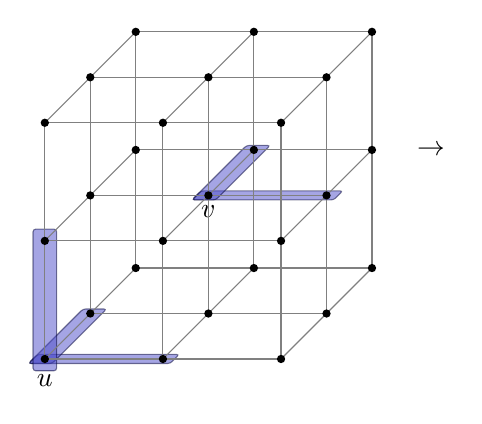
\begin{tikzpicture}[scale=1.5]

\tikzset{xyp/.style={canvas is xy plane at z=#1}}
\tikzset{xzp/.style={canvas is xz plane at y=#1}}
\tikzset{yzp/.style={canvas is yz plane at x=#1}}

\draw[blue!20!black,fill=blue!70!black!70,rounded corners=1,opacity=0.5, xzp=1]%,shift={(0.15,0.15)}]
(0.9,1.1) rectangle (2.1,0.9);


      \draw[blue!20!black,fill=blue!70!black!70,rounded corners=1,opacity=0.5, xzp = 1]%,shift={(0.15,0.15)}]
      (0.9,1.1) rectangle (1.1,-0.1);



\draw[blue!20!black,fill=blue!70!black!70,rounded corners=1,opacity=0.5, xzp=0]%,shift={(0.15,0.15)}]
(-0.1,2.1) rectangle (1.1,1.9);


      \draw[blue!20!black,fill=blue!70!black!70,rounded corners=1,opacity=0.5, xzp = 0]%,shift={(0.15,0.15)}]
      (-0.1,2.1) rectangle (0.1, 0.9);

      \draw[blue!20!black,fill=blue!70!black!70,rounded corners=1,opacity=0.5, xyp = 2]%,shift={(0.15,0.15)}]
      (-0.1,-0.1) rectangle (0.1, 1.1);
%,opacity=0.5]
%\fill[blue!30]
%(0.8,0.8,1.2) -- (0.7,0.7,0) -- (2,2,0) -- (2,2,1.2) -- cycle;
%
%\fill[blue!30]
%(0.9,0.9,1.1) -- (0.9,0.9,-0.1) -- (1.1,0.9,-0.1) -- (1.1,0.9,1.1) -- cycle;  

      \node[below] at (1,1,1) { $v$ } ;
      \node[below = 2pt] at (0,0,2) { $u$ } ;

% draw grid lines
\foreach \x in {0,1,2} {
  \foreach \y in {0,1,2} {
    \draw[gray] (\x,\y,0) -- (\x,\y,2);
  }
}

\foreach \x in {0,1,2} {
  \foreach \z in {0,1,2} {
    \draw[gray] (\x,0,\z) -- (\x,2,\z);
  }
}

\foreach \y in {0,1,2} {
  \foreach \z in {0,1,2} {
    \draw[gray] (0,\y,\z) -- (2,\y,\z);
  }
}

% draw lattice points
\foreach \x in {0,1,2} {
  \foreach \y in {0,1,2} {
    \foreach \z in {0,1,2} {
      \fill (\x,\y,\z) circle (1pt);
    }
  }
}

\draw (2.5,1) node { $\rightarrow$ };
\end{tikzpicture} 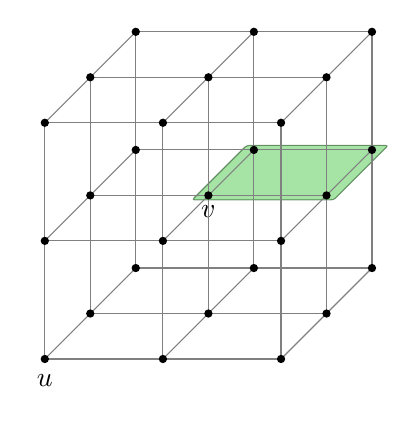
\begin{tikzpicture}[scale=1.5]

\tikzset{xyp/.style={canvas is xy plane at z=#1}}
\tikzset{xzp/.style={canvas is xz plane at y=#1}}
\tikzset{yzp/.style={canvas is yz plane at x=#1}}

      \draw[green!20!black,fill=green!70!black!70,rounded corners=1,opacity=0.5, xzp = 1]%,shift={(0.15,0.15)}]
      (0.9,1.1) rectangle (2.1,-0.1);


      \node[below] at (1,1,1) { $v$ } ;
      \node[below = 2pt] at (0,0,2) { $u$ } ;

% draw grid lines
\foreach \x in {0,1,2} {
  \foreach \y in {0,1,2} {
    \draw[gray] (\x,\y,0) -- (\x,\y,2);
  }
}

\foreach \x in {0,1,2} {
  \foreach \z in {0,1,2} {
    \draw[gray] (\x,0,\z) -- (\x,2,\z);
  }
}

\foreach \y in {0,1,2} {
  \foreach \z in {0,1,2} {
    \draw[gray] (0,\y,\z) -- (2,\y,\z);
  }
}

% draw lattice points
\foreach \x in {0,1,2} {
  \foreach \y in {0,1,2} {
    \foreach \z in {0,1,2} {
      \fill (\x,\y,\z) circle (1pt);
    }
  }
}
\end{tikzpicture}
  \caption{SWEEP rule}
  \label{fig:sweep}
\end{figure}




The way we quantify the 'perimeter' of an error cluster is by considering the (hyper)triangle that bounds the vertices supporting the cluster. Now, the poles of an error cluster are the vertices that lie on the sides of the triangle. We followed \cite{Berman}, and by embedding the Toric in the infinite plane, we were able to identify the poles as the max/min points of linear functions which we call \textit{potential walls}. Then, we show that the sweep rule advances only one pole - matching the corner mentioned earlier. And hence, advances one side, forward the others.
As a consequence, a sweep-cycle decreases the sides of the bounding triangle, and hence the 'perimeter'. 


The embedding restricts periodicity conditions on the assignments. We encounter this twice: first, an assignment on the Toric's faces that closes a non-trivial cycle translates to an infinite assignment in the infinite plane. In that case, no triangle bounds the error, which agrees with the fact that a logical error—in that context, an error that changes the logical states—should be 'decoded' to a different codeword. From a technical perspective, it comes into effect as the claims about shrinking assume that a given assignment is a connected finite assignment (or a collection of connected components such that each of them is finite).
The second time we have to deal with the mapping onto the infinite plane is in the calculation of the probability of a given Toom's contour to occur.
Since different leaves (faults) of Toom's contour might be associated with the same qubit\footnote{Actually, the leaves are vertices that support the face associated with a faulty qubit.} and hence dependent, to bypass this, we took from \cite{gacs2021newversiontoomsproof} the claim that states any such graph has a subgraph whose leaves are independent, and their number is at least a constant factor of the original leaves.
    \begin{figure}[H]

\begin{center}
    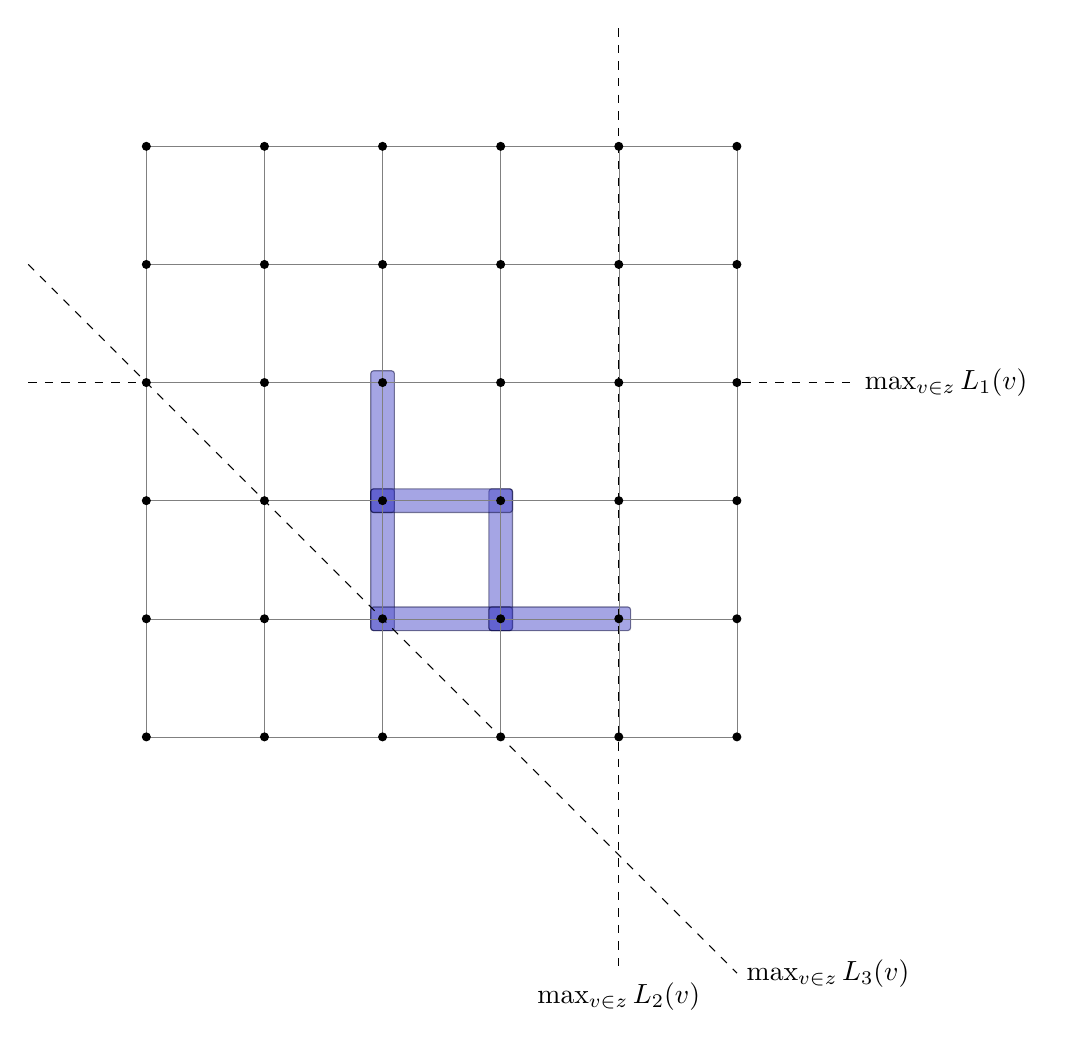
\begin{tikzpicture}[scale=1.5]


  \draw[blue!20!black,fill=blue!70!black!70,rounded corners=1, opacity=0.5]%shift={(0.15,0.15)}]
  (1.9,0.9) 
  rectangle (2.1,2.1);


  \draw[blue!20!black,fill=blue!70!black!70,rounded corners=1, opacity=0.5]%shift={(0.15,0.15)}]
  (2.9,0.9) 
  rectangle (3.1,2.1);
  \draw[blue!20!black,fill=blue!70!black!70,rounded corners=1, opacity=0.5]%shift={(0.15,0.15)}]
  (1.9,1.9) 
  rectangle (2.1,3.1);


  \draw[blue!20!black,fill=blue!70!black!70,rounded corners=1, opacity=0.5]%,shift={(0.15,0.15)}]
  (1.9,0.9) 
  rectangle (3.1,1.1);

  \draw[blue!20!black,fill=blue!70!black!70,rounded corners=1, opacity=0.5]%,shift={(0.15,0.15)}]
  (1.9,1.9) 
  rectangle (3.1,2.1);
  \draw[blue!20!black,fill=blue!70!black!70,rounded corners=1, opacity=0.5]%,shift={(0.15,0.15)}]
  (2.9,0.9) 
  rectangle (4.1,1.1);
  \draw[dashed] (-1,3) -- (6,3) node[right] { $\max_{v \in z }L_{1}(v)$ };
  \draw[dashed] (4,6) -- (4,-2) node[below] { $\max_{v \in z} L_{2}(v)$ };
  \draw[dashed] (-1,4) -- (5,-2) node[right] { $\max_{v \in z} L_{3}(v)$ };

  \draw[step=1cm,gray,very thin] (0,0) grid (5,5);
  \foreach \x in {0,1,2,3,4,5}
  \foreach \y in {0,1,2,3,4,5}
  {
  \node[draw,circle,inner sep=1pt,fill] at (\x,\y) {};
}


\end{tikzpicture}
\end{center}
\caption{
A graphical example of the maximal values of the potential walls. Here we consider the $(2,1)$-Toric code, namely the bits are set on the edges where the $Z$-stabilizers (parity checks) are set on the vertices. The grid is a finite $6\times 6$ patch of the infinite 2D plane. The edges marked in blue correspond to a bits assignment $z$. Each of the dashed lines marks the line of vertices whose $L_{i}$ value converges with the maximal value reached by a vertex in $z$. Moving into the infinite plane enables us to determine those lines and draw the triangle that bounds $z$.
}
\label{fig:potwall}
\end{figure}



See \Cref{subsection:infinitetoric} for embedding into the infinite plane, \Cref{subsection:shrink} for the proof of shrinking, and \Cref{subsection:separator} for the claim about the existence of a sufficient subgraph. 


\paragraph{The Intermediate Argument.}
%\label{subsection:internediate}
Now that we have the code and decoder, the next difference we have to address is how to classify an error. Unlike the classical regime, flipping a stabilizer's qubits doesn't count as a fault. Moreover, the sweep-rule discussed above doesn't shrink stabilizers (as it acts trivially on them). Therefore, we need to redefine what is considered a divergence from the ideal computation. To overcome it, we define the reduced form of an error to be its translation by stabilizer that minimizes the 'perimeter' of the bounding triangle. Then we prove that the poles of the error in it's reduced coalesce with the poles of the syndrome it induces. In particular, the proof that the sweep-rule shrinks an error (\Cref{subsection:shrink}) assumes that the given error is in its reduced form. As a result, instead of defining the vertices of Toom's contour graph to be the flipped vertices as in \cite{Berman}, we define them to be qubits\footnote{In fact: vertices on the qubits' support, see \Cref{subsection:toricencoded}.} in the reduced form of the error.

We then face another challenge: if we analyze Toom's contour, which is induced by the single time unit running consisting of flipping all the qubits at once, then in the layer following the fault cycle, even though the error contains many qubits, its reduced form is empty. In the language of Toom's contour, as will be defined later, the Toom's contour is empty, and no bounds on the event's probability to occur can be inferred using it. 
More generally, there is a threshold, such that for errors exceeding that threshold, one cannot restore the history of the error. In fact, the threshold is far lower than flipping all the qubits and matching errors that close a non-trivial cycle.

We address this by introducing an analysis framework where all computation, including faults, is imagined to occur sequentially — in steps. Within this framework, we can prove an \textit{intermediate claim} stating that on the path to an error configuration closing a non-trivial cycle, one must pass through a step with an error where the 'perimeter' its reduced form is large. Thus, a sufficient condition for a logical error to occur in some time unit is the existence of a step with a reduced error that is large.  
Moreover, having such a step implies the existence of a step for which it happens for the first time, meaning that prior to that, no error has closed a non-trivial cycle, the sweep-rule worked as it should, and a Toom's contour describing the history of the error can be constructed. Thus, an upper bound on the probability of the condition can be derived. In the proof of the theorem, we show that this condition happens with negligible probability. To elaborate on the issue, we first need to present the computation model.

We model a noisy running of a given circuit $C$ as follows: first, we sample space-time locations for the faults and denote the outcome by $\mathcal{E}$. Then, we impose layers of computation alternately, such that the even and odd layers are taken from $\mathcal{E}$ and $C$ according to their order. The combination of the circuit $C$ with a subset of faults $\mathcal{E}$ defines a possible running, and we call it a subjection of $C$ to $\mathcal{E}$ and denote it by $C[\mathcal{E}]$. Furthermore, we showed in \Cref{claim:block_noise_renorm} that for a local-stochastic noise model, unbalancing partition to noisy and logical layers, for example placing a noisy layer after every three logical layers of $C$, is equivalent to odd-even alternations up to a rescaling of the noise rate (by a constant). We use that since the error correction cycle of the sweep rule takes more than a single layer.



\begin{figure}[htbp]
  \begin{minipage}[c]{0.6\textwidth}
  \centering
\begin{quantikz}
\lstick{$\ket{0}$} & \gate{H} &  & \ctrl{1} &   \\
\lstick{$\ket{0}$} & \gate{H} & \gate{\inr{X}} & \gate{S} &  & \ctrl{1} \\
\lstick{$\ket{0}$} & \gate{H} & \gate{\inr{X}} & \ctrl{1} &  & \targ{} \\
\lstick{$\ket{0}$} & \gate{H} &  & \targ{} & \gate{\inr{X}} & 
\end{quantikz}
\end{minipage}%
  \begin{minipage}[c]{0.3\textwidth}
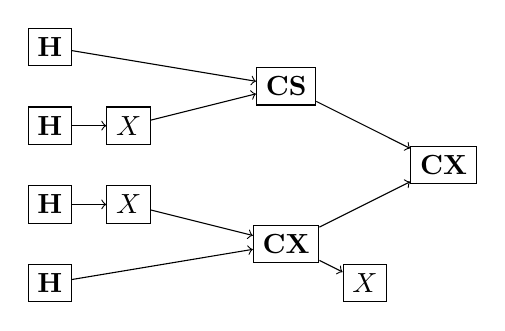
\begin{tikzpicture}
  \node[rectangle,draw] (A)  at (0,3) { $\mathbf{H}$ }; 
  \node[rectangle,draw] (B)  at (0,2) { $\mathbf{H}$ }; 
  \node[rectangle,draw] (C)  at (0,1) { $\mathbf{H}$ }; 
  \node[rectangle,draw] (D)  at (0,0) { $\mathbf{H}$ }; 
  \node[rectangle,draw] (E) at (1,2) { $\inr{X}$ } ; 
  \node[rectangle,draw] (F) at (1,1){ $\inr{X}$ }  ; 
  \node[rectangle,draw] (G)  at (3,2.5) { $\mathbf{CS}$ }; 
  \node[rectangle,draw] (H)  at (3,0.5) { $\mathbf{CX}$ }; 
  \node[rectangle,draw] (I)  at (4,0) { $\inr{X}$ }; 
  \node[rectangle,draw] (J)  at (5,1.5) { $\mathbf{CX}$ }; 
  \draw[->] (B) to (E);
  \draw[->] (C) to (F);
  \draw[->] (A) to (G);
  \draw[->] (E) to (G);
  \draw[->] (F) to (H);
  \draw[->] (D) to (H);
  \draw[->] (H) to (I);
  \draw[->] (G) to (J);
  \draw[->] (H) to (J);
\end{tikzpicture}
\end{minipage}
\caption{  Example of a subjected quantum circuit: the even layers (0, 2, 4) contain the original gates, while the faults are imposed on the odd layers and marked in red. }
  \label{fig:examplecirc}
\end{figure}

As mentioned, we are going to analyze the likelihood of getting logical errors by looking back in time and asking what a run that has led to them is supposed to look like. The sweep rule ensures that an error cluster below a certain size, sufficiently low to not closing a non-trivial cycle, shrinks. 
The problem is that a single fault layer (i.e., a layer whose source is in $\mathcal{E}$) might increase the error cluster above that size. At first glance, one might be tempted to show that the expansion of error clusters beyond a fraction of the code distance happens with negligible probability, but that calculation soon becomes complicated when considering the merging of disjoint clusters. 
Here comes the splitting of the computation into steps to advantage. In each step, only one gate or one fault is applied, and steps are ordered such that they agree with the computation. Figure \ref{fig:examplecirc} illustrates a quantum circuit and a graph of steps corresponding to it.


Since the gates and the faults have a bounded fan-in/out\footnote{The faults are bounded-fan because we can assume that in the time units representation they are Pauli products and therefore in the steps presentation they are decomposed into single qubit Pauli matrices.} In each step, the maximal size of an error cluster can increase by at most a constant factor, with the maximal increase occurring when multiple clusters are merged. Equipped with that insight, we are able to infer the intermediate argument. 


\Cref{subsection:model} formalize the computation model and the computation graph presentation (splitting to steps). In addition, see \Cref{claim:intersyn} for the formal proof of the intermediate argument. 

\paragraph{Description of the Construction.}
Similarly to other fault tolerance approaches, we use the concatenation construction \cite{aharonov1999faulttolerant} in order to initialize zeros and resource states encoded in the 4D-Toric code, as referred to in \cite{grospellier:tel-03364419}, \cite{gottesman2014faulttolerant}. From there, we assume that all the quantum registers are encoded in the 4D-Toric code, and we name each of the encoded block a quantum register. The resources states are spread across two registers.


Then, after the initialization step, the logical cycles are divided into error correction, which is a single sweep-cycle, and 'logical operation' cycle. For our universal logical gate set, we choose $ \mathbf{X}, \mathbf{Z}, \mathbf{CX}$ (controlled NOT), $\mathbf{H}$, $\mathbf{S}$, and $\mathbf{T}$ gates. Except for the Paulis and the 'Controlled NOT' gate, which are realized by transversal Paulis and transversal wire-wise physical 'Controlled NOT' gates, all the others are implemented via gate teleportation \cite{Zhou_2000}.

The general realization by gate teleportation is done as follows: first, we XOR the target state into a resource state via $\mathbf{CX}$, measure the input state and the first register of the resource state with a Bell measurement, the input register in the $X$ basis, and the first register of the resource state in the $Z$ basis. Then, on the classical outcomes, run a classical decoding procedure to extract the logical codeword. Meanwhile, on the second register of the resource, which is intended to contain the result of the action, perform a sweep cycle. At the end of the decoding, depending on the result, we apply either a transversal Pauli operator or the $\mathbf{S}$ gate (again by teleportation) depending on the original gate that was asked to simulate. The gate teleportation lasts for multiple logical cycles, depending on the depth required by the classical decoding procedure.


We emphasize that for measuring the input register in the $X$-basis, we apply the Hadamard through its fold-transversal realization \cite{Breuckmann_2024}, so the measurement is done in constant depth. However, the reason we don't implement the Hadamard by fold-transversal from the beginning is that it introduces an expansion in the bounded-triangle by the fold-transversal realization. Since it guarantees that after the measurement the register will not observe more faults, we can tolerate a one-time blowup in the size of the error and still be able to decode the logical state in the register correctly. Yet, for the Clifford-free depth overhead, we do use the fold-transversal implementation followed by sufficiently many followed sweep-cycles. As a result, we stretch the depth of the basic logical layer, which in turn comes into effect by a lower threshold for the noise rate.

In \Cref{subsection:logical}, we discuss in detail the structures of the logical codeword of the $(d,d^{\prime})$-Toric code and the realization of its logical gates.


\paragraph{Toom's Contours.} 
A sufficiently simple definition of Toom's contours in \cite{Berman} would be a directed graph that describes a noisy run with the additional marking of diverged bits. In our case —the quantum case— the vertices of Toom's contour are neither bits nor checks; instead, they are the vertices on the Torices that 'diverged'. A proper conceptual definition would be:
\begin{center}
\begin{minipage}{0.75\textwidth}
  \textit{
A graph that describes a noisy run from the Torices' perspective. In particular, the vertices of the graph are the vertices of the Torices, equipped with a time coordinate, that witness a faulty qubit in a reduced form.
  }
\end{minipage}
\end{center}
We adjust their construction as follows: Denote the graph by $\mathcal{H} \colonequals (V_{\mathcal{H}}, E_{\mathcal{H}})$ and by $P_{1},..,P_{t}$ a \textit{Pauli-path}, such that $P_{i}$ is the propagated error up to time $i$ (including faults that occur at that time), and each 'cluster' of error in $P_{i}$ is in its reduced form. Then,
\begin{enumerate}
  \item  If at time $t$, a vertex $v$ on one of the Toric complexes\footnote{Actually the infinite grid.} corresponding to one of the quantum registers supports a face -qubit- that belongs to a reduced error, then add $(v,t)$ to the vertices.
  \item If at time $t$, vertex $v$ belongs to a reduced error, and at time $t+1$ its neighbor $u$ belongs to a reduced error, then we think of the situation as '$v$ "leads" to $u$' and connect $(v,t)$ and $(u,t+1)$ with an "arrow." The vertices $v$ and $u$ might belong to different registers (which matches the case that at time $t$ we apply an operator on both registers). For convenience, we don't require $u$ at time $t$ to belong only to non-faulty qubits.
  \item As in the classical case, connect any two vertices in $V_{\mathcal{H}}$ that are connected to a third by 'arrows' with a 'fork'.
\end{enumerate}


\begin{figure}[h]
  \centering
  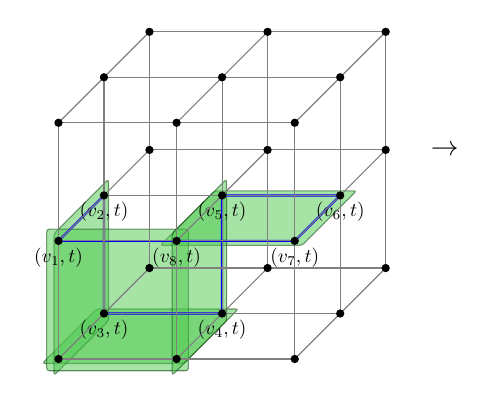
\begin{tikzpicture}[scale=1.5]

\tikzset{xyp/.style={canvas is xy plane at z=#1}}
\tikzset{xzp/.style={canvas is xz plane at y=#1}}
\tikzset{yzp/.style={canvas is yz plane at x=#1}}



\draw[green!20!black,fill=green!70!black!70,rounded corners=1,opacity=0.5, xzp=0]%,shift={(0.15,0.15)}]
(-0.1,2.1) rectangle (1.1,0.9);

\draw[green!20!black,fill=green!70!black!70,rounded corners=1,opacity=0.5, xzp=1]%,shift={(0.15,0.15)}]
(0.9,2.1) rectangle (2.1,0.9);

      \draw[green!20!black,fill=green!70!black!70,rounded corners=1,opacity=0.5, yzp = 0]%,shift={(0.15,0.15)}]
      (-0.1,2.1) rectangle (1.1, 0.9);


      \draw[green!20!black,fill=green!70!black!70,rounded corners=1,opacity=0.5, xyp = 2]%,shift={(0.15,0.15)}]
      (-0.1,-0.1) rectangle (1.1, 1.1);
      

      \draw[green!20!black,fill=green!70!black!70,rounded corners=1,opacity=0.5, yzp = 1]%,shift={(0.15,0.15)}]
      (-0.1,2.1) rectangle (1.1, 0.9);
%,opacity=0.5]
%\fill[green!30]
%(0.8,0.8,1.2) -- (0.7,0.7,0) -- (2,2,0) -- (2,2,1.2) -- cycle;
%
%\fill[green!30]
%(0.9,0.9,1.1) -- (0.9,0.9,-0.1) -- (1.1,0.9,-0.1) -- (1.1,0.9,1.1) -- cycle;  



      \draw[blue, thick]  (0,1,2) -- (1,1,2); % -- (1,1,1);
      \draw[blue, thick] (0,1,1) -- (0,1,2) -- (0,1,1) -- (0,0,1) -- (1,0,1) -- (1,1,1) -- (2,1,1) -- (2,1,2) -- (1,1,2);


      \node[below , scale=0.7] at (0,1,2) { $(v_{1}, t)$ } ;
      \node[below , scale=0.7] at (0,1,1) {$(v_{2}, t)$} ;
      \node[below , scale=0.7] at (0,0,1) {$(v_{3}, t)$} ;
      \node[below , scale=0.7] at (1,0,1) {$(v_{4}, t)$} ;
      \node[below , scale=0.7] at (1,1,1) {$(v_{5}, t)$} ;
      \node[below , scale=0.7] at (2,1,1) {$(v_{6}, t)$} ;
      \node[below , scale=0.7] at (2,1,2) {$(v_{7}, t)$} ;
      \node[below , scale=0.7] at (1,1,2) {$(v_{8}, t)$} ;
% draw grid lines
\foreach \x in {0,1,2} {
  \foreach \y in {0,1,2} {
    \draw[gray] (\x,\y,0) -- (\x,\y,2);
  }
}

\foreach \x in {0,1,2} {
  \foreach \z in {0,1,2} {
    \draw[gray] (\x,0,\z) -- (\x,2,\z);
  }
}

\foreach \y in {0,1,2} {
  \foreach \z in {0,1,2} {
    \draw[gray] (0,\y,\z) -- (2,\y,\z);
  }
}

% draw lattice points
\foreach \x in {0,1,2} {
  \foreach \y in {0,1,2} {
    \foreach \z in {0,1,2} {
      \fill (\x,\y,\z) circle (1pt);
    }
  }
}

\draw (2.5,1) node { $\rightarrow$ };
\end{tikzpicture} 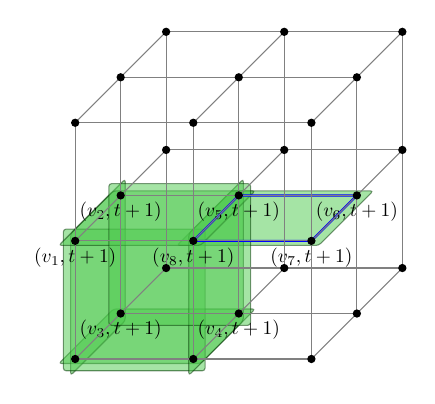
\begin{tikzpicture}[scale=1.5]

\tikzset{xyp/.style={canvas is xy plane at z=#1}}
\tikzset{xzp/.style={canvas is xz plane at y=#1}}
\tikzset{yzp/.style={canvas is yz plane at x=#1}}



\draw[green!20!black,fill=green!70!black!70,rounded corners=1,opacity=0.5, xzp=0]%,shift={(0.15,0.15)}]
(-0.1,2.1) rectangle (1.1,0.9);

\draw[green!20!black,fill=green!70!black!70,rounded corners=1,opacity=0.5, xzp=1]%,shift={(0.15,0.15)}]
(0.9,2.1) rectangle (2.1,0.9);

      \draw[green!20!black,fill=green!70!black!70,rounded corners=1,opacity=0.5, yzp = 0]%,shift={(0.15,0.15)}]
      (-0.1,2.1) rectangle (1.1, 0.9);


      \draw[green!20!black,fill=green!70!black!70,rounded corners=1,opacity=0.5, xyp = 2]%,shift={(0.15,0.15)}]
      (-0.1,-0.1) rectangle (1.1, 1.1);
      

      \draw[green!20!black,fill=green!70!black!70,rounded corners=1,opacity=0.5, yzp = 1]%,shift={(0.15,0.15)}]
      (-0.1,2.1) rectangle (1.1, 0.9);

\draw[green!20!black,fill=green!70!black!70,rounded corners=1,opacity=0.5, xzp=1]%,shift={(0.15,0.15)}]
(-0.1,2.1) rectangle (1.1,0.9);

      \draw[green!20!black,fill=green!70!black!70,rounded corners=1,opacity=0.5, xyp = 1]%,shift={(0.15,0.15)}]
      (-0.1,-0.1) rectangle (1.1, 1.1);


      \draw[blue, thick]  (1,1,1) -- (2,1,1) -- (2,1,2) -- (1,1,2) -- (1,1,1);

      \node[below , scale=0.7] at (0,1,2) { $(v_{1}, t+1)$ } ;
      \node[below , scale=0.7] at (0,1,1) {$(v_{2}, t+1)$} ;
      \node[below , scale=0.7] at (0,0,1) {$(v_{3}, t+1)$} ;
      \node[below , scale=0.7] at (1,0,1) {$(v_{4}, t+1)$} ;
      \node[below , scale=0.7] at (1,1,1) {$(v_{5}, t+1)$} ;
      \node[below , scale=0.7] at (2,1,1) {$(v_{6}, t+1)$} ;
      \node[below , scale=0.7] at (2,1,2) {$(v_{7}, t+1)$} ;
      \node[below , scale=0.7] at (1,1,2) {$(v_{8}, t+1)$} ;

% draw grid lines
\foreach \x in {0,1,2} {
  \foreach \y in {0,1,2} {
    \draw[gray] (\x,\y,0) -- (\x,\y,2);
  }
}

\foreach \x in {0,1,2} {
  \foreach \z in {0,1,2} {
    \draw[gray] (\x,0,\z) -- (\x,2,\z);
  }
}

\foreach \y in {0,1,2} {
  \foreach \z in {0,1,2} {
    \draw[gray] (0,\y,\z) -- (2,\y,\z);
  }
}

% draw lattice points
\foreach \x in {0,1,2} {
  \foreach \y in {0,1,2} {
    \foreach \z in {0,1,2} {
      \fill (\x,\y,\z) circle (1pt);
    }
  }
}
\end{tikzpicture}


  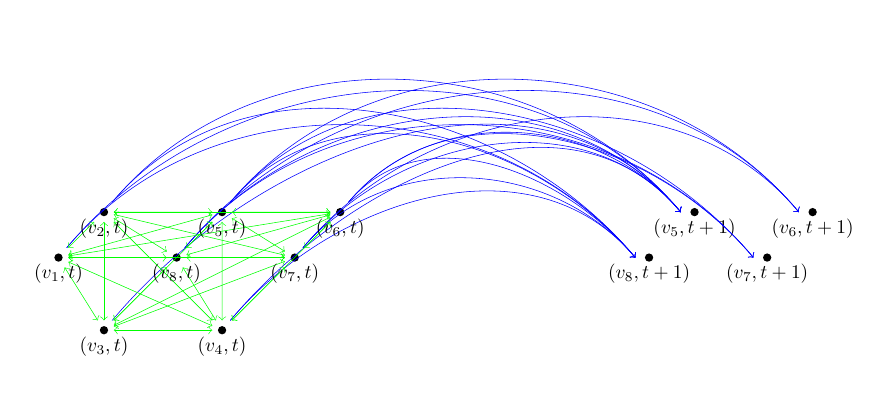
\begin{tikzpicture}[scale=1.5]

\tikzset{xyp/.style={canvas is xy plane at z=#1}}
\tikzset{xzp/.style={canvas is xz plane at y=#1}}
\tikzset{yzp/.style={canvas is yz plane at x=#1}}





\node(A) at (0,1,2) {} ;
\node(B) at (0,1,1) {} ;
\node(C) at (0,0,1) {} ;
\node(D) at (1,0,1) {} ;
\node(E) at (1,1,1) {} ;
\node(F) at (2,1,1) {} ;
\node(G) at (2,1,2) {} ;
\node(H) at (1,1,2) {} ;


      \fill (0,1,2) circle(1pt)  ;
      \fill (0,1,1) circle(1pt) ;
      \fill (0,0,1) circle(1pt) ;
      \fill (1,0,1) circle(1pt) ;
      \fill (1,1,1) circle(1pt) ;
      \fill (2,1,1) circle(1pt) ;
      \fill (2,1,2) circle(1pt) ;
      \fill (1,1,2) circle(1pt) ;
% draw grid lines

% draw lattice points
\foreach \x in {0,1,2} {
  \foreach \y in {0,1,2} {
    \foreach \z in {0,1,2} {
      \node at (\x,\y,\z) { } ;
    }
  }
}


\node[below , scale=0.7](I) at (5,1,1) {$(v_{5}, t+1)$} ;
\node[below , scale=0.7](J) at (6,1,1) {$(v_{6}, t+1)$} ;
\node[below , scale=0.7](K) at (6,1,2) {$(v_{7}, t+1)$} ;
\node[below , scale=0.7](L) at (5,1,2) {$(v_{8}, t+1)$} ;
 
\draw[blue,very thin,-> ]  (A) to [out=50, in=130] (I); 
\draw[blue,very thin,-> ]  (A) to [out=50, in=130] (L);
\draw[blue,very thin,-> ]  (B) to [out=50, in=130] (I); 
\draw[blue,very thin,-> ]  (B) to [out=50, in=130] (L);
\draw[blue,very thin,-> ]  (C) to [out=50, in=130] (I); 
\draw[blue,very thin,-> ]  (D) to [out=50, in=130] (I); 
\draw[blue,very thin,-> ]  (D) to [out=50, in=130] (L);
\draw[blue,very thin,-> ]  (E) to [out=50, in=130] (J); 
\draw[blue,very thin,-> ]  (E) to [out=50, in=130] (L);
\draw[blue,very thin,-> ]  (E) to [out=50, in=130] (K); 


\draw[blue,very thin,-> ]  (H) to [out=50, in=130] (I); 
\draw[blue,very thin,-> ]  (H) to [out=50, in=130] (K);
\draw[blue,very thin,-> ]  (H) to [out=50, in=130] (J); 

\draw[blue,very thin,-> ]  (F) to [out=50, in=130] (I); 
\draw[blue,very thin,-> ]  (F) to [out=50, in=130] (L);
\draw[blue,very thin,-> ]  (F) to [out=50, in=130] (K); 

\draw[blue,very thin,-> ]  (G) to [out=50, in=130] (I); 
\draw[blue,very thin,-> ]  (G) to [out=50, in=130] (L);
\draw[blue,very thin,-> ]  (G) to [out=50, in=130] (J); 

\draw[green,very thin,<-> ]  (A) to (B); 
\draw[green,very thin,<-> ]  (A) to (C); 
\draw[green,very thin,<-> ]  (A) to (D); 
\draw[green,very thin,<-> ]  (A) to (E); 
\draw[green,very thin,<-> ]  (A) to  (H);
\draw[green,very thin,<-> ]  (A) to  (G);
\draw[green,very thin,<-> ]  (A) to  (F);

\draw[green,very thin,<-> ]  (B) to (C); 
\draw[green,very thin,<-> ]  (B) to (D); 
\draw[green,very thin,<-> ]  (B) to (E); 
\draw[green,very thin,<-> ]  (B) to  (H);
\draw[green,very thin,<-> ]  (B) to  (G);
\draw[green,very thin,<-> ]  (B) to  (F);


\draw[green,very thin,<-> ]  (C) to (D); 
\draw[green,very thin,<-> ]  (C) to (E); 
\draw[green,very thin,<-> ]  (C) to  (H);
\draw[green,very thin,<-> ]  (C) to  (G);
\draw[green,very thin,<-> ]  (C) to  (F);

\draw[green,very thin,<-> ]  (D) to (E); 
\draw[green,very thin,<-> ]  (D) to  (H);
\draw[green,very thin,<-> ]  (D) to  (G);
\draw[green,very thin,<-> ]  (D) to  (F);

\draw[green,very thin,<-> ]  (E) to  (H);
\draw[green,very thin,<-> ]  (E) to  (G);
\draw[green,very thin,<-> ]  (E) to  (F);


\draw[green,very thin,<-> ]  (F) to  (H);
\draw[green,very thin,<-> ]  (F) to  (G);

\draw[green,very thin,<-> ]  (H) to  (G);


      \fill (5,1,1) circle(1pt) ;
      \fill (6,1,1) circle(1pt) ;
      \fill (6,1,2) circle(1pt) ;
      \fill (5,1,2) circle(1pt) ;

\node[below , scale=0.7] at (0,1,2) { $(v_{1}, t)$ } ;
\node[below , scale=0.7] at (0,1,1) {$(v_{2}, t)$} ;
\node[below , scale=0.7] at (0,0,1) {$(v_{3}, t)$} ;
\node[below , scale=0.7] at (1,0,1) {$(v_{4}, t)$} ;
\node[below , scale=0.7] at (1,1,1) {$(v_{5}, t)$} ;
\node[below , scale=0.7] at (2,1,1) {$(v_{6}, t)$} ;
\node[below , scale=0.7] at (2,1,2) {$(v_{7}, t)$} ;
\node[below , scale=0.7] at (1,1,2) {$(v_{8}, t)$} ;




% draw grid lines

% draw lattice points
      \foreach \x in {4,5,6} {
  \foreach \y in {0,1,2} {
    \foreach \z in {0,1,2} {
      \node at  (\x,\y,\z) { };
    }
  }
}
\end{tikzpicture}


\caption{
Above: The application of a sweep-cycle, where the green faces represent the bits assignment $z$, and the blue edges correspond to unsatisfied checks $\partial^{-} z$. The vertices witnessing a syndrome, namely belonging to $\partial^{-}z$, are labeled as $v_{1}, v_{2}, \ldots, v_{8}$. Notice that the leftmost bottom-inner vertex is not witnessing a syndrome even though it belongs to $z$. Below: The Toom's contour derived from the single computation layer that matches the cycle. Arrows are colored in blue, while forks are colored in green. Note that $(v_{1}, t+1)$ doesn't belong to the Toom's contour (since $v_{1}$ doesn't see an unsatisfied check at time $t+1$).
}
  \label{fig:toomscontours}
\end{figure}

Later, we incorporate the 'splitting into turns' idea into the formation of Toom's counter $\mathcal{H}$-graphs, by gluing the layers corresponding to the first $t-1$ layers with a final layer that matches a partial execution of the $t$th time unit. The layer encodes the situation of the running up to a certain step. Then, combining with the intermediate theorem, we have that any running that admits a logical error derives a Toom's contour, with sufficiently large vertices at final layer. 


The rest of the analysis follows \cite{Berman}. We define \textit{slices} at time $t$ to be connected (by arrows) components of vertices at time $t$. Then, in the merging of two slices into one, it is guaranteed that faults induced by each are disjoint; otherwise, those two slices will be connected by arrows, namely - the same slice. For a \textit{slice}, we define its size to be the perimeter of the triangle that would bound the vertices of the slice if they were projected on the same Toric. Then, by induction, we prove that Toom's contour that induces at time $t$ a slice with size $s$ has a spanning tree with at most and at least a constant times $s$ edges and leaves (and therefore faults). That allows us to bound the probability of such a slice occurring by counting the number of possible spanning trees and assigning them the probability that the minimal number of faults occurs.

One technical change that we made and haven't discussed yet is that in the gluing of the last layer, which was defined to capture a partial layer execution up to a turn, we connect by arrows any two vertices that were added to $ V_{\mathcal{H}} $ and share a check. By doing so, we ensure that connected components in the bits-to-checks graph would also be connected by arrows in Toom's contours. That is necessary since, without the last gluing, an error cluster that closes a non-trivial loop on the Toric might consist of two 'connected by arrows' error clusters which are tangent.
We emphasize that such edges connection can be made only in the last stage, as it doesn't pass the induction step. However, the final slice that is formed passes the desired inequalities only by constants and is therefore sufficiently good to derive the probability bound.

\Cref{subsection:toricencoded} defines Toom's contours, \Cref{subsection:spacetimegraph} defines the slices and states a claim connecting a slice to its predecessors, and \Cref{subsection:explantion} provides the induction proofs.

%\section{The Proof in Detail}



%That can be thought as an adaptation  Gacs and Reif ideas \cite{GACS1988125}, Where the $n$-logical bit corresponds to colony, in their approach corrections done via the Toom's rule which is uniform for all the bits. 



  \subsection{ Notations } \label{sec:nota}
We follow the standard notations commonly used in the literature. For an integer $n$, we denote by $[n]$ the set of integers $\{1, 2, \ldots, n\}$. To present a countable set, which might or might not be finite, where the number of elements does not matter, we use curly brackets with a subscript denoting the first index of the set. For example, $\{u_{i}\}_{i=1}$ represents the set $u_{1}, u_{2}, \ldots$. For finite sets, we might add a superscript to present the size of the set. If the first index is clear from the context, then we might omit the assignment.
We use a colon inside curly brackets to specify a set of elements satisfying a condition, i.e., for sets $A, B$, the notation $\{ a : a \in A, a \in B \}$ equals $A \cap B$. Curly brackets without subscripts or conditions refer to singletons. For example, for a given integer $i$, the set $\{u_{i}\}$ is the set that contains only the element $u_{i}$. For an integer $i$, we denote by $1_{i}$ the vector consisting of one at the $i$th coordinate and zero elsewhere. The char $|$ symbolizes a restriction, for example $x|_{y}$, is the restriction of the 'entity $x$' to '$y$'. The particular behavior of the restriction would change depending on the target type.

When not otherwise mentioned, we consider quantum states over qubits, each lying in a two-dimensional Hilbert space $\mathcal{H}_{2}$, and denote by $\mathcal{H}_{2^n}$ the Hilbert space of an $n$-qubit system. The $\otimes$ operator stands for tensor product, for example: $\mathcal{H}_{2^n} = \mathcal{H}_{2}^{\otimes n}$. The space of linear operators on the Hilbert space is denoted by $L(\mathcal{H})$.  Pure quantum states and their dual presentations are denoted by $\ket{\psi}, \bra{\psi}$, and in the matrix representation, we use $\ket{\psi}\bra{\psi}$ to denote its density matrix. We will use $\rho$ to denote a mixed state. The letters, $X$ and $Z$, will usually denote the single qubit $X$ and $Z$ Pauli operators. Yet, where the Pauli matrices are out of context, we use these letters for other variables. The gate 'Controlled Not' is denoted by $\mathbf{CX}$, and the gates Hadamard, S, and T are denoted by:
\begin{equation*}
  \begin{split}
    \mathbf{H} = \frac{1}{\sqrt{2}}\begin{bmatrix}
      1 & 1 \\
      1 & -1 
    \end{bmatrix}, \mathbf{S} = \begin{bmatrix}
      1 & 0 \\
      0 & i 
    \end{bmatrix}, \mathbf{T} = \begin{bmatrix}
      1 & 0 \\
      0 & e^{i\frac{\pi}{4}} 
    \end{bmatrix}
  \end{split}
\end{equation*}
For a quantum gate $U$, we denote by $\ket{U}$ the resource state that can be used to simulate $U$. Notice that, in general, the resource state is not unique. In this work, we address specific states that will be discussed later. 

\iffalse 

  We use $\mathcal{N} : L(\mathcal{H}) \rightarrow L(\mathcal{H})$ to denote a $p$-local stochastic noise channel, namely a channel in which for any subset $S$ of the (qu)bits, the probability that all the qubits in $S$ absorb noise is less than $p^{|S|}$. We recall that for a constant-depth circuit, when the fanout/in of its subgates is bounded, one can map the running of the circuits subjected to $p$-local stochastic noise to a running when the states are subjected only to $p^{\prime}$-local stochastic noise before entering the circuit, and then the rest of the computation is done in an ideal environment \cite{gottesman2014faulttolerant}, where $p^{\prime}$ is a function of $p$ and constants. If the gate is also a measure, for example as a decoder, then the mapping induces also $q$-local stochastic noise on the measurements.

  \begin{figure}[h]
  \label{fig:noise}
  \begin{center}
  \begin{quantikz}[row sep=0.3cm, column sep=0.7cm]
    \lstick{$q_1$} & \gate[wires=8]{U_0} & \gate{\mathcal{N}} & \gate[wires=8]{U_1}   & \gate{\mathcal{N}} & \gate[wires=8]{U_2} & \gate{\mathcal{N}}& \qw \\
    \lstick{$q_2$} &                      & \gate{\mathcal{N}} &                      & \gate{\mathcal{N}} &                     & \gate{\mathcal{N}} & \qw \\
    \lstick{$q_3$} &                      & \gate{\mathcal{N}} &                      & \gate{\mathcal{N}} &                     & \gate{\mathcal{N}} & \qw \\
    \lstick{$q_4$} &                      & \gate{\mathcal{N}} &                      & \gate{\mathcal{N}} &                     & \gate{\mathcal{N}} & \qw \\
    \lstick{$q_5$} &                      & \gate{\mathcal{N}} &                      & \gate{\mathcal{N}} &                     & \gate{\mathcal{N}} & \qw \\
    \lstick{$q_6$} &                      & \gate{\mathcal{N}} &                      & \gate{\mathcal{N}} &                     & \gate{\mathcal{N}} & \qw \\
    \lstick{$q_7$} &                      & \gate{\mathcal{N}} &                      & \gate{\mathcal{N}} &                     & \gate{\mathcal{N}} & \qw \\
    \lstick{$q_8$} &                      & \gate{\mathcal{N}} &                      & \gate{\mathcal{N}} &                     & \gate{\mathcal{N}} & \qw
  \end{quantikz}
  \caption{ Circuit subjected to noise. }

  \end{center}
\end{figure}

We think about computation subjected to noise as the running of a circuit, in which at any time, qubits might be 'flipped', or formally, with some constant probability, they are replaced with the fully mixed state. Since our computation might create correlations between the errors, we will assume nothing about the behavior of the errors except that big errors are unlikely. By doing that, the induction step doesn't have to guarantee the errors being uncorrelated. 

We use \Cref{def:pnoise} to describe the running of a circuit subjected to noise. \Cref{fig:noise} illustrates a noisy circuit. In the figure, the channel $N$ acts on each qubit separately, yet this is not the case, and we impose it in that way only to make a clear distinction between the original gates and the noise channels. \begin{definition}{$p$-Noisy Circuit.}
    \label{def:pnoise}
    Given a circuit $C$ (regardless of the model), its $p$-noisy version $\tilde{C}$ is the circuit obtained by alternately taking layers from $C$ and then passing each (qu)bit through a $p$-local stochastic channel.
  \end{definition}

  
  Generally speaking, we say that a decision problem is solvable by a uniform family of circuits $\mathcal{C}$ if there is a polynomial $poly : \mathbb{R} \rightarrow \mathbb{R}$, such that for any large enough $n \in \mathbb{N}$, there exist $a, b \in (0,1)$ at a distance of at least $b - a > 1/\text{poly}(n)$ and a polynomial Turing machine $M$ such that for any given instance $x$ with encoding length $|x| = n$, the running of $M$ on $x$ outputs $C_x \in \mathcal{C}$ that, when running over the zero word $0^{*}$, induces on the first (qu)bit at least $b$ probability to be at $1$ if $x$ is in the language and at most $a$ to be at $1$ otherwise. 
If a decision problem is solvable by a $p$-noisy version of $C \in \mathcal{C}$, we say that the problem is solvable by noisy-$\mathcal{C}$. We abuse the notation, and for complexity class $Q$, we define noisy-$Q$ to be all the decision problems solvable by the noisy version of the circuit family that solves the problems in $Q$. For example, noisy-\textbf{BQP} is the class of all the decision problems solvable by noisy polynomial quantum circuits.  


The first class we are interested in is Nick's Class, $\NC{}$  characterizing the boolean circuits at logarithmic depth. This class was proven by Pippenger to be equal to its noisy version, namely noisy-$\NC{} = \NC{}$ \cite{Pippenger}. Formally defined as follows: 
\begin{definition}[$\NC{}$ - Nick's Class]
$\NC_i$ is the class of decision problems solvable by a uniform family of Boolean circuits, with polynomial size, depth $O(\log^i(n))$, and fan-in $2$. 
\end{definition}


Second, the analog class of $\NC{}$ is $\QNC{}$, which characterizes logarithmic depth quantum circuits. In $\QNC{}$, the circuits are also allowed to have any single qubit gate. While in the classical case the number of functions from $\{0,1\}^{2} \rightarrow \{0,1\}$ is finite, in the quantum case we have an infinite number of single gates. That motivated us to define $\QNCG{}$ - the circuits when the gate set is restricted to some finite, constant size group $G$. We emphasize that in \textbf{BQP} there is no point in restricting to such a family since any gate can be polynomially approximated at polylogarithmic depth, so in that case, the restriction does not change computational power and one can assume to be able to apply any single qubit gate. However, when considering shallow circuits at logarithmic depth, such assumptions don't hold anymore.
\begin{definition}[$\QNC{}$]
  The class of decision problems solvable by polynomial size,  polylogarithmic-depth,  and finate fan out/in quantum circuits with bounded probability of error. Similarly to $\NC_i{}$, $\QNC_i{}$ is the class where the decisdes the circuits have $\log^i (n)$ depth.  
\end{definition}

\begin{definition}[$\QNCG{}$]
  For a fixing finate fan in/out gateset $G$, the class with deciding circuits at polynomial size, composed only for gates in $G$ and at depth at most polylogaritmic. And in similar to $\QNC_{i}{}$, $\QNCiG{}$ is the restriction to circuits with depth at most $\log^{i}(n)$.  
\end{definition}

Another setting which we find interesting is the equipping of classes with an unbounded fanout CNOT gate, a gate which acts as $\ket{x}\prod_{i}\ket{y_{i}} \rightarrow \ket{x}\prod_{i}\ket{x \oplus y_{i}}$. There are two main reasons we find those class worth considering. First, the unbounded fanout CNOT can be decomposed by chaining only two-qubit CNOTs, since for any CSS code, a CNOT can be implemented in a fault-tolerant manner almost for free. Second, there are candidates at $\QNCzef$ for proving quantum advantage\cite{Bremner_2017}, \cite{Paletta_2024}.


\begin{definition}[$\QNCzef{}$] 
Similarly to $\QNCze{}$, the class of decision problems solvable by constant depth and bounded fan out/in quantum circuits equipped additionally with a 'quantum fanout' gate is available, which CNOTs a qubit into arbitrarily many target qubits in a single step.
\end{definition}

Finally, the last setting we consider is the restriction of the classes when there is no access to fresh qubits, or equivalently, no reset gates are allowed. In this setting, any step of computation accumulates entropy, and an exponential trade-off relation between entropy and depth was proved.

\begin{definition}[$\QNCon{}$ without reset gates.]
  The class of decision problems solvable by polynomial size,  logarithmic-depth, and finate fan out/in quantum circuits with bounded probability of error, without reset gates.
\end{definition}
Those definitions lead us to ask our first open problem:
\begin{oproblem}[The Main Open Problem.]
\begin{equation*}
  \begin{split}
    \text{ Does }  \QNCon{} = \text{ noisy-}\QNCon{} \text{?}
  \end{split}
\end{equation*}
\end{oproblem}
Our second main problem investigates whether it matters which universal gateset is used for the simulation, or whether the answer to the previous question is affirmative when our computation is restricted to a finite gateset $G^{\prime}$, given that the source was also restricted to using local computation in a finite set. That is, we ask: \begin{oproblem}[Constant Depth Overhead on $G^{\prime}$ Restricted Machine.]
  Does there exist a finite universal set $G^{\prime}$ such that for any finite two-qubit gateset $G$ it holds that:
\begin{equation*}
  \begin{split}
\QNCG{}_{,1} = \text{noisy-}\QNC{}_{\mathbf{G^{\prime}}, 1} \text{?}
  \end{split}
\end{equation*}
\end{oproblem}

In this context, we mention the work of \cite{kim2025catalyticzrotationsconstanttdepth}, which shows that using a catalyst state\footnote{In the catalytic computation model, one has access to a complicated resource state $\ket{\phi}$, yet he has to return/keep it at the end of the running.}, no bounded fan-out computation can simulate any single qubit gate with a constant $T$ depth. Namely, in our words, they prove that there exists a finite gate set $G^{\prime}$ such that:
\begin{equation*}
  \begin{split}
    \QNC{}_{f,1} = \QNC{}_{f, \mathbf{G^{\prime}}, 1} \text{ using catalyst state. }
  \end{split}
\end{equation*}
We hope that our work will also lead to an understanding of the importance, or the non-importance, of the basic components being used.


\fi
 

\label{subsection:model}
\newcommand{\comDAG}{\pi_{C[\mathcal{E}]}} 
\paragraph{The Computation Model.} Informally, a quantum circuit is a placement of a collection of quantum gates, taken from a finite set, at different space-time locations. Each such location records when the gate is applied and on which qubits it acts. Formally:

\begin{definition}[Quantum Circuit]
  \label{def:quantcirc}
  A \emph{space-time location} is a pair $l=(t,S)$, where $t$ is a time coordinate and $S=(s_{1},\ldots,s_{\Delta})$ is an ordered tuple of qubit indices. For a finite collection of quantum gates
  \begin{equation*}
    \begin{split}
      \mathcal{G} \subset \Big\{ g \colon L(\mathcal{H}_{2}^{\otimes \Delta}) \to L(\mathcal{H}_{2}^{\otimes \Delta}) \Big\},
    \end{split}
  \end{equation*}
  and integers $w,d\in\mathbb{N}$, a quantum circuit $C$ of depth $d$ and width $w$ is a collection of tuples
  \begin{equation*}
    \begin{split}
      C=\{u_i=(g_i,l_i)\}_i,
    \end{split}
  \end{equation*}
  where each $g_i\in\mathcal{G}$ and each location $l_i=(l_{i,1},l_{i,2})$ belongs to $[d]\times [w]^{\Delta}$. We call the tuples $u_i$ \textit{the gates of $C$}. They must satisfy the following compatibility condition: if two gates have the same time coordinate, then their supports are disjoint. Namely, for $u_i=(g_i,l_i),u_j=(g_j,l_j)\in C$, the equality $l_{i,1}=l_{j,1}$ implies that the sets of qubit indices appearing in $l_{i,2}$ and $l_{j,2}$ are disjoint. We denote by
  \begin{equation*}
    \begin{split}
      \operatorname{Loc}(C) \colonequals \{l_i : u_i=(g_i,l_i)\in C\}
    \end{split}
  \end{equation*}
  the set of locations occupied by the gates of $C$. We define the \textit{$t$-layer} of $C$ to be its restriction to gates at time $t$:
  \begin{equation*}
    \begin{split}
      C|_{t} \colonequals \{u_i=(g_i,l_i)\colon u_i\in C \text{ and } l_{i,1}=t\}.
    \end{split}
  \end{equation*}
\end{definition}
Later, we will restrict $\mathcal{G}$ to contain $\mathbf{CX}, \mathbf{H}, \mathbf{S}, \mathbf{T}$, and measurements. To define the action of a quantum circuit $C$ on a given mixed state, we first associate $C$ with a directed acyclic graph.
\begin{definition}[Associated Computation DAG]
  \label{def:steps}
  Let $C=\{u_i\}_i$ be a quantum circuit with depth $d$ and width $w$. We define the associated computation DAG of $C$, denoted by $\pi_C$, to be the directed acyclic graph $\pi_C=(\mathcal{U},E)$ as follows:
  \begin{enumerate}
    \item The vertex set is the gate set of $C$, namely $\mathcal{U}=\{u_i\}_i$.
    \item For $u_i=(g_i,l_i)$ and $u_j=(g_j,l_j)$, there is a directed edge $(u_i,u_j)\in E$ if and only if $j$ is one of the minimizers of
      \begin{equation*}
        \begin{split}
          \big\{ l_{k,1} : (g_k,l_k)\in \mathcal{U},\ l_{k,1}>l_{i,1},\ l_{k,2}\cap l_{i,2}\neq\emptyset \big\}.
        \end{split}
      \end{equation*}
      Equivalently, $u_j$ is one of the earliest later gates whose support intersects the support of $u_i$. There may be more than one such minimizer, so the out-degree may exceed one.
  \end{enumerate}

  Suppose that $J=(j_1,j_2,\ldots,j_k)$ is an ordering of the gate indices that agrees with a topological order induced by $\pi_C$. Then we define the associated partial circuits $C_J=\{C_{J,i}\}_{i=1}^{k}$ by
  \begin{enumerate}
    \item $C_{J,1}=\{u_{j_1}\}$.
    \item For $1\le i<k$, set $ C_{J,i+1}=C_{J,i}\cup\{u_{j_{i+1}}\}$.
  \end{enumerate}
      We call $C_{J,i}$ the partial computation circuit up to step $i$.
\end{definition}

\begin{definition}
  Let $\rho$ be a density matrix over $w$ qubits, and let $C = \{u_{i}\}_{i=1}$ be a quantum circuit with depth $d$ and width $w$. For any density matrix $\sigma$, quantum gate $g \in \mathcal{G}$, and location $l$, the application of the gate-location tuple $(g,l)$ on $\sigma$, denoted by $(g,l) \circ \sigma$, is the application of $g$ on $\sigma$ where wires are ordered such that the first qubit in the input to $g$ is $l_{2,1}$, the second is $l_{2,2}$, and so on. The result of the application of $C$ on $\rho$, denoted by $C \circ \rho$, is given by iterative applications of the gates $\{u_{i}\}_{i=1}$ on $\rho$, according to a topological order induced by $\pi_{C}$.

We say that $\rho_{1}, \rho_{2}, \ldots, \rho_{k}$ is a computation prefix if $\rho_{1} = \rho$ and $\rho_{i+1} = u^\prime_{i} \circ \rho_{i}$, where $\{u^{\prime}_{i}\}_{i=1}$ is a prefix of a topological ordering of $\{u_{i}\}_{i=1}$. If $\{u^{\prime}_{i}\}_{i=1}$ contains all the gates in $\{u_{i}\}_{i=1}$, then we call $\rho_{1}, \rho_{2}, \ldots, \rho_{k}$ a running.
\end{definition}
For a quantum circuit $C$, we would like to discuss its action in the presence of different outcomes of faults. The following definition encodes the running in the presence of a specific set of faults $\mathcal{E}$.
%We do this by defining a new circuit, stacking a layer of $\mathcal{E}$ after every $m$ layers of $C$.
\begin{definition}[$C$ subjected to $\mathcal{E}$ every $m$ computational layers]
  Let $C=\{u_i\}_i$ be a quantum circuit with depth $d$ and width $w$, let $m\in\mathbb{N}$, and set
  \begin{equation*}
    \begin{split}
      d_m \colonequals \left\lceil \frac{d}{m} \right\rceil.
    \end{split}
  \end{equation*}
  Let $\mathcal{L}\subset [d_m]\times [w]$ be a set of locations, and let $\mathcal{E}$ be a quantum circuit, such $\text{Loc}(\mathcal{E}) = \mathcal{L}$. We name $\mathcal{E}$ \textit{subsets of faults}, and we name the layers of $\mathcal{E}$ \textit{fault layers}.
  The circuit \textit{$C$ subjected to $\mathcal{E}$ every $m$ computational layers}, denoted by $C[\mathcal{E}]_{m}$, is obtained by setting the first layer to be the first layer of $\mathcal{E}$, then placing in order the layers of $C$ and inserting one fault layer after every $m$ consecutive $C$'s layers. Thus the second fault layer is inserted after the layers $1,\ldots,m$ of $C$, the third is inserted after the layers $m+1,\ldots,2m$ of $C$, and so on. Concretely, each gate $u_i=(g_i,(t_i,S_i))$ of $C$ is moved to the time coordinate
  \begin{equation*}
    \begin{split}
      t_i + \left\lfloor \frac{t_i-1}{m} \right\rfloor,
    \end{split}
  \end{equation*}
  while each fault gate $(g,(t,S))\in\mathcal{E}$ is placed at time coordinate
  \begin{equation*}
    \begin{split}
      t(m+1).
    \end{split}
  \end{equation*}
  When $m=1$, the gates occupy the even time coordinates and the fault layers occupy the odd time coordinates. When the parameter is omitted, we mean $m=1$. We denote the associated computation DAG of $C[\mathcal{E}]_{m}$ by $\comDAG$.
\end{definition}





\begin{remark}
  Formally, a fault circuit is just a particular quantum circuit whose gates are interpreted as faults rather than as computational operations. Thus the distinction between a quantum circuit and a fault circuit is semantic rather than structural: both are circuits in the sense of \Cref{def:quantcirc}, but they play different roles in the analysis.
\end{remark}

\begin{example}
  When $m=3$, the 'computational' layers are sent to the times
  \begin{equation*}
    \begin{split}
      2,3,4,6,7,8,10,11,12,\ldots,
    \end{split}
  \end{equation*}
  while the fault layers are sent to the times
  \begin{equation*}
    \begin{split}
      1,5,9,13,\ldots.
    \end{split}
  \end{equation*}
\end{example}
Later, all the quantum registers will be encoded via stabilizer codes. Then, following the common approach in the literature, we define the fault layers to end with stabilizer measurements, thereby forcing the faults to be Paulis (see \cite{gottesman1997stabilizercodesquantumerror}). Hence, we confine ourselves to noise channels of only this type.
\begin{definition}[Noise channel and local stochastic noise channel]
  \label{def:localstoc}
  A \textit{noise channel} $\mathcal{N}_{\mathcal{E}}$ is a distribution over sets of faults and their locations. Let $p\in(0,1)$, we say that the noise channel $\mathcal{N}_{\mathcal{E}}$ is \textit{local stochastic with rate $p$} if for every finite set of locations $S\subset \mathbb{N}\times \mathbb{N}$,
  \begin{equation*}
    \begin{split}
      \prbm{S\subset \operatorname{Loc}(\mathcal{E})}{\mathcal{E}\sim \mathcal{N}_{\mathcal{E}}}
      \le p^{|S|}.
    \end{split}
  \end{equation*}
Through this work, the sampled faults will be assumed to be Pauli.
\end{definition}
So, $N_{\mathcal{E}}$ defines a probability space. The set of faults $\mathcal{E}$ is an atomic outcome, and for a given circuit $C$, the subjected circuit $C[\mathcal{E}]$ is a random variable. The following claim states that for local stochastic noise, the subjection of every 1-layer is equivalent to the subjection of every $m$-layer, up to a rescaling of the noise rate. Here, by equivalence, we mean that the actions of the subjected circuits are the same\footnote{For a given input (mixed) state $\rho$, they yield the same output}. We give the proof in the appendix (see, \Cref{claim:block_noise_renorm_app}). 
\begin{claim}
  \label{claim:block_noise_renorm}
  Let $\mathcal{N}_{\mathcal{E}}$ be a local stochastic noise channel with rate $p$, and let $C$ be a quantum circuit whose gates have arity at most $\Delta$. Fix an even integer $c$. Then there exists a local stochastic noise channel $\mathcal{N}_{\mathcal{E}_{q}}$ with rate
  \begin{equation*}
    \begin{split}
      q \colonequals \left(2^{H(\Delta^{-2c})\Delta^{2c}}p\right)^{\Delta^{-c}},
    \end{split}
  \end{equation*}
  such that for any given state $\rho$ it holds that:
  \begin{equation*}
    \begin{split}
      C[\mathcal{E}]_{1} \circ \rho =  C[\mathcal{E}_{q}]_{c/2} \circ \rho
    \end{split}
  \end{equation*}
  In particular, up to a constant depending only on $\Delta$ and $c$, the rate $q$ behaves like $p^{\Delta^{-c}}$.
\end{claim}
Equipped with this claim, we are allowed to assume having constant depth cycles that don't observe faults. 

\begin{definition}
  Let $C$ be a quantum circuit that contains $l$ measurements. For possible outcomes $\alpha \in \mathbb{F}^{l}_{2}$, let $C[,\alpha]$ be the circuit obtained by conditioning that $\alpha_{1},..,\alpha_{l}$ were measured. We extend the notation for the subjected circuit by denoting $C[\mathcal{E},\alpha]$ as the subjected circuit where the measurements are assumed to outcome $\alpha_{1},..,\alpha_{l}$.
\end{definition}
 

\inb{\textbf{ Write here something. }} 
\begin{remark}
  \label{remark:condmeas}
  Consider the presentation of a conditioned circuit as a subset of gates acting on locations. For an outcome $\alpha \in \mathbb{F}_{2}^{(\cdot)}$ for which a conditional gate (for example, a $\mathbf{CCZ}$, where the control bits are conditioned on measurement outcomes) in the original circuit $C$ is mapped to a Pauli in $C[,\alpha]$, we substitute this gate with the Pauli on the target tensored with identity acting on the control locations. Thus, the order of the steps, the locations of each gate, and the computation graph of $C[,\alpha]$ are the same as for $C$ (and independent of the outcomes). We summarize this by briefly saying that the locations are invariant to the conditioning of measurements. 
\end{remark}

In our case, the conditioned circuit $C[\mathcal{E}, \alpha]$ is a Clifford circuit; in particular, it sends Paulis to Paulis. That brings us to define, for a given set of faults $\mathcal{E}$ and outcomes $\alpha$, a Pauli-path that describes the evolution of the faults through the circuit. 


\begin{definition}[Propagation]
  \label{def:propagation}
  Let $C[\mathcal{E}]$ be a subjected quantum circuit at depth $\mu$, and let $\alpha \in \mathbb{F}_{2}^{(\cdot)}$ be a possible outcome vector for $C[\mathcal{E}]$. Suppose that $C$ is a Clifford+measurements circuit, so $C[\mathcal{E},\alpha]$ is a Clifford circuit. We define the propagation of Pauli $P \in \mathcal{P}$ through the conditioned circuit $C[\mathcal{E},\alpha]$ to be the Paulis $P_{1}, \ldots, P_{\mu+1}$ such that $P_{1} = P$ and for any $i \in [2, \mu+1]$:
  \begin{equation*}
    \begin{split}
      P_{i}C[,\alpha]|_{\rightarrow i} =  C[\mathcal{E},\alpha]|_{ i} P_{i-1} C[,\alpha]|_{\rightarrow i-1} = C[\mathcal{E},\alpha]|_{\rightarrow i}P_{1}
    \end{split}
  \end{equation*}
We extend the notation to step-propagation by considering the propagation of the circuit obtained from $C[\mathcal{E},\alpha]$ by flattening the circuit such that each gate is applied at the time that equals its step. 
\end{definition}




\subsection{Time Coarse-Graining}



The following claim states that for local stochastic noise, the subjection of every 1-layer is equivalent to the subjection of every $m$-layer, up to a rescaling of the noise rate. Here, by equivalence, we mean that the actions of the subjected circuits are the same\footnote{For a given input (mixed) state $\rho$, they yield the same output}. We give the proof in the appendix (see, \Cref{claim:block_noise_renorm_app}). 
\begin{claim}
  \label{claim:block_noise_renorm}
  Let $\mathcal{N}_{\mathcal{E}}$ be a local stochastic noise channel with rate $p$, and let $C$ be a quantum circuit whose gates have arity at most $\Delta$. Fix an even integer $c$. Then there exists a local stochastic noise channel $\mathcal{N}_{\mathcal{E}_{q}}$ with rate
  \begin{equation*}
    \begin{split}
      q \colonequals \left(2^{H(\Delta^{-2c})\Delta^{2c}}p\right)^{\Delta^{-c}},
    \end{split}
  \end{equation*}
  such that for any given state $\rho$ it holds that:
  \begin{equation*}
    \begin{split}
      C[\mathcal{E}]_{1} \circ \rho =  C[\mathcal{E}_{q}]_{c/2} \circ \rho
    \end{split}
  \end{equation*}
  In particular, up to a constant depending only on $\Delta$ and $c$, the rate $q$ behaves like $p^{\Delta^{-c}}$.
\end{claim}




\inb{ \textbf{ Say somthing about that we assume that the gates are uniteris, otherwise the propagation does not work. } }


In this section, we prove that when subjecting a Clifford + measurements circuit to local stochastic noise, changing the frequency at which we introduce the fault layers translates to rescaling the noise rate. For this purpose, we are abusing the notation "propagation" by reusing it to describe a different context.
\begin{definition}[Layer propagation]
  Let $C = \{u_{i}\}_{i=1}$ be a quantum Clifford circuit. For each time coordinate $t$, write $U_{t}\colonequals C|_{t}$. The family of non-empty $t$-cuts $\{U_{t}\}_{t}$ is called the \textit{layer decomposition} of $C$.

  Let $t<t'$ be such that $U_t$ and $U_{t'}$ are non-empty and $U_s=\emptyset$ for every $t<s<t'$. The \textit{forward propagation} of the layer $U_{t}$ across the next layer $U_{t'}$ is the operation that replaces the pair $(U_{t},U_{t'})$ by a pair $(U_{t'},V_{t\to t'})$ satisfying
  \begin{equation*}
    \begin{split}
      \prod_{u\in U_{t}}u\prod_{v\in U_{t'}}v
      =
      \prod_{v\in U_{t'}}v\prod_{w\in V_{t\to t'}}w.
    \end{split}
  \end{equation*}
  The layer $V_{t\to t'}$ is called the \textit{propagation expression} of $U_{t}$ across $U_{t'}$.

  More generally, if $t<t'$, the \textit{forward propagation of $U_t$ to time $t'$} is obtained by iterating the above operation through the successive non-empty cuts between times $t$ and $t'$. The resulting propagated layer is denoted by $V_{t\to t'}$ and is again called the propagation expression of $U_t$ to time $t'$. The resulting circuit has layer decomposition
  \begin{equation*}
    \begin{split}
      \ldots,U_{t-1},U_t,U_{t+1},\ldots,U_{t'},U_{t'+1},\ldots
      \mapsto
      \ldots,U_{t-1},U_{t+1},\ldots,U_{t'},V_{t\to t'},U_{t'+1},\ldots.
    \end{split}
  \end{equation*}
  After propagation we update the time coordinates so that they agree with the new layer in which each gate is applied.
\end{definition}


\begin{definition}[$C\sim_{P}C'$]
  For quantum circuits $C$ and $C'$, we write $C\sim_{P}C'$ if one can be obtained from the other by a finite sequence of layer propagations.
\end{definition}

By construction, $\sim_{P}$ preserves the implemented channel. Indeed, if $C\sim_{P}C'$ and $\rho$ is any mixed state on the input register, then
\begin{equation*}
  \begin{split}
    C\circ \rho = C'\circ \rho.
  \end{split}
\end{equation*}

We state \Cref{claim:block_noise_renorm} in the language of layer propagation.
\begin{claim}
  \label{claim:block_noise_renorm_app}
  Let $\mathcal{N}_{\mathcal{E}}$ be a local stochastic noise channel with rate $p$, and let $C$ be a quantum circuit whose gates have arity at most $\Delta$. Fix an even integer $c$. Then there exists a local stochastic noise channel $\mathcal{N}_{\mathcal{E}_{q}}$ with rate
  \begin{equation*}
    \begin{split}
      q \colonequals \left(2^{H(\Delta^{-2c})\Delta^{2c}}p\right)^{\Delta^{-c}},
    \end{split}
  \end{equation*}
  such that $C[\mathcal{E}]_{1} \sim_{P} C[\mathcal{E}_{q}]_{c/2}$. In particular, up to a constant depending only on $\Delta$ and $c$, the rate $q$ behaves like $p^{\Delta^{-c}}$.
\end{claim}
\begin{proof}[Proof of \Cref{claim:block_noise_renorm}]
  Partition the subjected circuit $C[\mathcal{E}]_{1}$ into consecutive blocks of $c$ layers. Inside each block, propagate all the fault layers to the end of the block and then groupping the resultd expressions together. Doing this block by block yields a new circuit $C^{\prime}$ in which each block of $c/2$ computational layers is followed by a single fault layer. Therefore $C^{\prime} = C[\mathcal{E}^{\prime}]_{c/2}$ for a suitable random fault set $\mathcal{E}^{\prime}$, and by construction: $C[\mathcal{E}]_{1} \sim_{P} C[\mathcal{E}']_{c/2}$. 
  


It remains to be proven that $\mathcal{E}^{\prime}$ is distributed according to a local stochastic channel. Fix one propagation expression $V^{(i)}$ and a subset $S \subset \operatorname{Loc}(V^{(i)})$. Denote by $U_{1}^{i}, \ldots, U_{c}^{i}$ the layers for which $V^{(i)}$ is their (grouped) expression. Denote the light cone of $S$ in $U_{1}^{i}, \ldots, U_{c}^{i}$ by $\Lambda(S)$. Since the fan is bounded by $\Delta$, we have that $|\Lambda(S)| \le \Delta^{c}|S|$, and any $S^{\prime} \subset \Lambda(S)$ whose propagation covers $S$ has size at least $|S^{\prime}| \ge \Delta^{-c}|S|$, and in particular contains a subset of size exactly $\Delta^{-c}|S|$.
  
Now, having $S \subset \operatorname{Loc}(V^{(i)})$, implies that there is a minimal $S^{\prime}$ (the minimality is regarding inclusion) such that $S^{\prime} \subset \operatorname{Loc}(\mathcal{E})$. Denote by $\mathcal{W}(S)$ the set of such minimal $S^{\prime}$'s, and observe that its size is at most:
    \begin{equation*}
      \begin{split}
 |\mathcal{W}(S)| \le { \Delta^{c}|S| \choose \Delta^{-c}|S| } 
      \end{split}
    \end{equation*}
    Hence, using the fact that $\mathcal{E}$ is an outcome of local stochastic noise channel with a noise rate $p$ we have:
  \begin{equation*}
    \begin{split}
      \prb{S\subset \operatorname{Loc}(V^{(i)})} &= \sum_{\alpha}\prb{S\subset \operatorname{Loc}(V^{(i)}) | \alpha } \prb{ \alpha } \\
      &\le
      \sum_{\alpha}\prb{\bigcup_{S'\in \mathcal{W}(S|\alpha)}\{S'\subset \operatorname{Loc}(\mathcal{E})\}| \alpha } \prb{\alpha} \\
      &\le
      \sum_{\alpha}\sum_{S'\in \mathcal{W}(S|\alpha)} \prb{S'\subset \operatorname{Loc}(\mathcal{E}) | \alpha} \prb{\alpha} \\
      & \le { \Delta^{c}|S| \choose \Delta^{-c}|S| } p^{\Delta^{-c}|S| } \le \left(2^{H(\Delta^{-2c})\Delta^{2c}}p\right)^{|S|/\Delta^{c}}
      = q^{|S|}.
    \end{split}
  \end{equation*}
\end{proof}

\printbibliography
%\section{Appendix}




%
%\inb{Below, a semi proof that in CSS code partial correction $Z^{e} \rightarrow Z^{\hat{e}}$ doesn't add bit flip errors. It might adds a global phase. I should enter it in a section about CSS coding. }
%
%\begin{equation*}
%  \begin{split}
%     & X^{f}Z^{e} \ket { w + C_{z}^{\perp} } \\
%     = & X^{f}Z^{e}X^{w} \ket { C_{z}^{\perp} } \\
%     \text{apply } H^{\otimes n } \mapsto & Z^{f}X^{e}Z^{w}\ket { C_{z} } \\
%     = & (-1)^{e \cdot w} Z^{f}Z^{w}X^{e}\ket { C_{z} } \\
%     \text{ partial correction } X^{e +\hat{e}} \mapsto & (-1)^{(e+\hat{e}) (f+w) } (-1)^{e \cdot w} Z^{f}Z^{w}X^{\hat{e}}\ket { C_{z} } \\
%     \text{apply } H^{\otimes n } \mapsto & (-1)^{(e+\hat{e}) (f+w) } (-1)^{e \cdot w} X^{f}X^{w}Z^{\hat{e}}\ket { C_{z}^{\perp} } \\
%     = & (-1)^{(e+\hat{e}) (f+w) } (-1)^{e \cdot w} (-1)^{\hat{e} \cdot w} X^{f}Z^{\hat{e}}X^{w}\ket { C_{z}^{\perp} } \\
%     = & (-1)^{(e+\hat{e}) f } X^{f}Z^{\hat{e}}\ket { w + C_{z}^{\perp}  } \\
%  \end{split}
%\end{equation*}
%
%
%\subsection{Base case for \Cref{claim:agreement}}
%\label{subsection:basecase}
%\begin{proof}
%
% The parity check matrices are:
%\setcounter{MaxMatrixCols}{40}
%\begin{equation*}
%  \begin{split}
%    H_{\mathcal{C}_{v}} = \begin{bmatrix}
%  1  &  1  &  1  &  0  &  0  &  0 \\
%  1  &  0  &  0  &  1  &  1  &  0 \\
%  0  &  1  &  0  &  1  &  0  &  1 \\
%  0  &  0  &  1  &  0  &  1  &  1
%\end{bmatrix} 
%\ \ \ \ \ H_{\text{Stab}_{v}} = \begin{bmatrix}
%  \inb{1}  &  \inb{1}  &  \inb{1}  &  0  &  0  &  0  &  0  &  0  &  0  &  0  &  0  &  0  &  0  &  0  &  0  &  0  &  0  &  0 \\
%  \inb{1}  &  0  &  0  &  \inb{1}  &  \inb{1}  &  0  &  0  &  0  &  0  &  0  &  0  &  0  &  0  &  0  &  0  &  0  &  0  &  0 \\
%  0  &  \inb{1}  &  0  &  \inb{1}  &  0  &  \inb{1}  &  0  &  0  &  0  &  0  &  0  &  0  &  0  &  0  &  0  &  0  &  0  &  0 \\
%  0  &  0  &  \inb{1}  &  0  &  \inb{1}  &  \inb{1}  &  0  &  0  &  0  &  0  &  0  &  0  &  0  &  0  &  0  &  0  &  0  &  0 \\
%  \inbr{1}  &  0  &  0  &  0  &  0  &  0  &  \inbr{1}  &  \inbr{1}  &  0  &  0  &  0  &  0  &  0  &  0  &  0  &  0  &  0  &  0 \\
%  0  &  \inbr{1}  &  0  &  0  &  0  &  0  &  \inbr{1}  &  0  &  \inbr{1}  &  0  &  0  &  0  &  0  &  0  &  0  &  0  &  0  &  0 \\
%  0  &  0  &  \inbr{1}  &  0  &  0  &  0  &  0  &  \inbr{1}  &  \inbr{1}  &  0  &  0  &  0  &  0  &  0  &  0  &  0  &  0  &  0 \\
%  \inbr{1}  &  0  &  0  &  0  &  0  &  0  &  0  &  0  &  0  &  \inbr{1}  &  \inbr{1}  &  0  &  0  &  0  &  0  &  0  &  0  &  0 \\
%  0  &  0  &  0  &  \inbr{1}  &  0  &  0  &  0  &  0  &  0  &  \inbr{1}  &  0  &  \inbr{1}  &  0  &  0  &  0  &  0  &  0  &  0 \\
%  0  &  0  &  0  &  0  &  \inbr{1}  &  0  &  0  &  0  &  0  &  0  &  \inbr{1}  &  \inbr{1}  &  0  &  0  &  0  &  0  &  0  &  0 \\
%  0  &  \inbr{1}  &  0  &  0  &  0  &  0  &  0  &  0  &  0  &  0  &  0  &  0  &  \inbr{1}  &  \inbr{1}  &  0  &  0  &  0  &  0 \\
%  0  &  0  &  0  &  \inbr{1}  &  0  &  0  &  0  &  0  &  0  &  0  &  0  &  0  &  \inbr{1}  &  0  &  \inbr{1}  &  0  &  0  &  0 \\
%  0  &  0  &  0  &  0  &  0  &  \inbr{1}  &  0  &  0  &  0  &  0  &  0  &  0  &  0  &  \inbr{1}  &  \inbr{1}  &  0  &  0  &  0 \\
%  0  &  0  &  \inbr{1}  &  0  &  0  &  0  &  0  &  0  &  0  &  0  &  0  &  0  &  0  &  0  &  0  &  \inbr{1}  &  \inbr{1}  &  0 \\
%  0  &  0  &  0  &  0  &  \inbr{1}  &  0  &  0  &  0  &  0  &  0  &  0  &  0  &  0  &  0  &  0  &  \inbr{1}  &  0  &  \inbr{1} \\
%  0  &  0  &  0  &  0  &  0  &  \inbr{1}  &  0  &  0  &  0  &  0  &  0  &  0  &  0  &  0  &  0  &  0  &  \inbr{1}  &  \inbr{1} \\
%  0  &  0  &  0  &  0  &  0  &  0  &  \inr{1}  &  0  &  0  &  \inr{1}  &  0  &  0  &  0  &  0  &  0  &  0  &  0  &  0 \\
%  0  &  0  &  0  &  0  &  0  &  0  &  0  &  \inr{1}  &  0  &  0  &  \inr{1}  &  0  &  0  &  0  &  0  &  0  &  0  &  0 \\
%  0  &  0  &  0  &  0  &  0  &  0  &  \inr{1}  &  0  &  0  &  0  &  0  &  0  &  \inr{1}  &  0  &  0  &  0  &  0  &  0 \\
%  0  &  0  &  0  &  0  &  0  &  0  &  0  &  0  &  \inr{1}  &  0  &  0  &  0  &  0  &  \inr{1}  &  0  &  0  &  0  &  0 \\
%  0  &  0  &  0  &  0  &  0  &  0  &  0  &  \inr{1}  &  0  &  0  &  0  &  0  &  0  &  0  &  0  &  \inr{1}  &  0  &  0 \\
%  0  &  0  &  0  &  0  &  0  &  0  &  0  &  0  &  \inr{1}  &  0  &  0  &  0  &  0  &  0  &  0  &  0  &  \inr{1}  &  0 \\
%  0  &  0  &  0  &  0  &  0  &  0  &  0  &  0  &  0  &  \inr{1}  &  0  &  0  &  \inr{1}  &  0  &  0  &  0  &  0  &  0 \\
%  0  &  0  &  0  &  0  &  0  &  0  &  0  &  0  &  0  &  0  &  0  &  \inr{1}  &  0  &  0  &  \inr{1}  &  0  &  0  &  0 \\
%  0  &  0  &  0  &  0  &  0  &  0  &  0  &  0  &  0  &  0  &  \inr{1}  &  0  &  0  &  0  &  0  &  \inr{1}  &  0  &  0 \\
%  0  &  0  &  0  &  0  &  0  &  0  &  0  &  0  &  0  &  0  &  0  &  \inr{1}  &  0  &  0  &  0  &  0  &  0  &  \inr{1} \\
%  0  &  0  &  0  &  0  &  0  &  0  &  0  &  0  &  0  &  0  &  0  &  0  &  0  &  \inr{1}  &  0  &  0  &  \inr{1}  &  0 \\
%  0  &  0  &  0  &  0  &  0  &  0  &  0  &  0  &  0  &  0  &  0  &  0  &  0  &  0  &  \inr{1}  &  0  &  0  &  \inr{1}
%\end{bmatrix}
%  \end{split}
%\end{equation*}
%Where we mark in \inb{blue}, \inbr{brown}, and \inr{red} the \inb{first}, \inbr{second}, and \inr{third} types of checks.
%
%
%\begin{equation*}
%  \begin{split}
%    G_{\mathcal{C}_{v}} =   \begin{bmatrix}
%  1  &  0  &  0 \\
%  0  &  1  &  0 \\
%  1  &  1  &  0 \\
%  0  &  0  &  1 \\
%  1  &  0  &  1 \\
%  0  &  1  &  1
%\end{bmatrix} \ \ \ \ \  \ \ \
%G_{\text{Stab}_{v}} = 
%\begin{bmatrix}
%  1  &  0  &  0  &  0 \\
%  0  &  1  &  0  &  0 \\
%  1  &  1  &  0  &  0 \\
%  0  &  0  &  1  &  0 \\
%  1  &  0  &  1  &  0 \\
%  0  &  1  &  1  &  0 \\
%  0  &  0  &  0  &  1 \\
%  1  &  0  &  0  &  1 \\
%  0  &  1  &  0  &  1 \\
%  0  &  0  &  0  &  1 \\
%  1  &  0  &  0  &  1 \\
%  0  &  0  &  1  &  1 \\
%  0  &  0  &  0  &  1 \\
%  0  &  1  &  0  &  1 \\
%  0  &  0  &  1  &  1 \\
%  1  &  0  &  0  &  1 \\
%  0  &  1  &  0  &  1 \\
%  0  &  0  &  1  &  1
%\end{bmatrix}
%  \end{split}
%\end{equation*}
%
%\end{proof}
%



%\subsection{Checks Commutation}
%We give an alternative proof of \Cref{claim:csscode} by straightforwardly multiplying checks. Consider subsets of generators $A, B \subset S$ with sizes $d^{\prime}-1$ and $d^{\prime}+1$, respectively. Thus, $\partial^{+} \rotfv{v}{A}$ and $\partial^{-} \rotfv{u}{B}$ are $X$- and $Z$-checks. Let us examine their multiplication:
%  \begin{equation*}
%    \begin{split}
%       ( \partial^{+} \rotfv{v}{A} ) ( \partial^{-} \rotfv{u}{B} )   = \left(\sum_{g \in S/A} \rotfv{v}{A \cup g} + \rotfv{g^{-1}v}{ A \cup g }\right)  \left(\sum_{g \in B} \rotfv{u}{B / g} + \rotfv{gu}{ B / g }\right) \\
%    \end{split}
%  \end{equation*}
%Split into cases based on whether $v$ equals $u$.
%\begin{enumerate}
%    \item If $v = u$, then for any $g, g^{\prime} \in S$, it holds that $gv \neq u$, $g^{\prime -1}u$, and $v \neq g^{\prime -1}u$. Thus, only terms of the form 
%\begin{equation*}
%  \begin{split}
%      \rotfv{v}{A \cup g}\rotfv{u}{B / g^{\prime}}
%  \end{split}
%\end{equation*}
%      can contribute to the product, yet for any $g, g^{\prime}$ for which this term is not zeroing out, it follows that $g \in B$ and $g^{\prime} \notin A$, and therefore the term 
%      \begin{equation*}
%        \begin{split}
%      \rotfv{v}{A \cup g^{\prime}}\rotfv{u}{B / g}
%        \end{split}
%      \end{equation*}
%      Is not zero as well. Therefore, the number of non-zero terms is even, namely the sum equals zero.
%
%    \item If there is $g$ such that $gv = u$, then first notice that for any $g^{\prime}, g^{\prime \prime} \in S/g \cup \{e\}$, we have $g^{\prime}v \neq u$. So only terms of the form 
%      \begin{equation*}
%        \begin{split}
%          \text{either } \rotfv{gv}{A \cup g}\rotfv{u}{B / g^{\prime}} \text{ or } \rotfv{v}{A \cup g^{\prime}}\rotfv{g^{-1}u}{B / g}
%        \end{split}
%      \end{equation*}
%      can contribute. Similarly to the above, if
%      \begin{equation*}
%        \begin{split}
%      \rotfv{gv}{A \cup g}\rotfv{u}{B / g^{\prime}} \neq 0
%        \end{split}
%      \end{equation*}
%       then $g \in B$ and $g^{\prime} \notin A$. So 
%       \begin{equation*}
%         \begin{split}
%       \rotfv{v}{A \cup g^{\prime}}\rotfv{g^{-1}u}{B / g}
%         \end{split}
%       \end{equation*}
%       is also not zeroing out, and again the number of non-zeros is even.
%\end{enumerate}
%
%
%\subsection{Infinite Compatibility}
%Here, we provide a proof that circuits for which an $\infty$-lift is defined are $\times$-compatible. Formally:
%\begin{claim} 
%\label{claim:infiequ}
%  Let $C$ be quantum circuit of the form defined in \Cref{def:extension}. Then $C$ is $\infty$-compatible.
%\end{claim}
%
%\begin{proof}
%Obviously, translation by the zero vector (or by the unit vertex) keeps the gate in its place, or in other words, in the restriction of $C^{\infty}$ to $[w]$ - the original Toric - any non-decoding gate is restored. We will need the following claim, which states that this is also true for a decoding gate.
%\begin{claim}
%\label{claim:pauli_back}
%Let $u = (g, l)$ be a decoding gate. The restriction of the image of $u$ in $C^{\infty}$ to $[w]$ is $u$ (when applied to the infinite domain). Namely:
%  \begin{equation*}
%    \begin{split}
%      \bigl(\prod_{a \in \mathbb{Z}^{d} } a *_{r} u \bigr)|_{[w]} = u
%    \end{split}
%  \end{equation*}
%\end{claim}
%\begin{proof}
%  Denote by $\hat{a}^{j} \in \mathbb{F}_{2}^{d}$ the vector which assigns in its $i$th coordinate $1$ if the root that supports the face of $u_{j}$ has a $g_{i}$ power greater than $n$. We argue that the $j$th face of $-\hat{a}^{j} *_{r} u$ is in $[w]$ and that the $j$th face of any other root translation of $u$ is not in $[w]$. That implies that the restriction
%  \begin{equation*}
%    \begin{split}
%      \bigl(\prod_{a \in \mathbb{Z}^{d} } a *_{r} u \bigr)|_{[w]}
%    \end{split}
%  \end{equation*}
%contains each of $u$'s faces exactly once, and combined with the fact that $u$ is a Pauli product, it follows that they are the same operator. 
%
%By the definition of root translation, we get that $(\hat{a}^{j} *_{r} u)_{j}$ is in $[w]$. Let $a^{\prime} \in \mathbb{Z}^{d}$ be such that $a^{\prime} \neq \hat{a}^{j}$, and denote by $i$ the coordinate on which they differ. Then, we get that the $g_{i}$ power of the root of $(a^{\prime} *_{r} u)_{j}$ is at a distance $n$ from the $g_{i}$ power of the root of $(\hat{a}^{j} *_{r} u)_{j}$; therefore, their roots can't both be in the range $[0,n-1]$, which implies that $(a^{\prime} *_{r} u)_{j} \notin [w]$.
%
%\end{proof}
%  From here we continue by induction on the number of the gates in $C$: 
%  \begin{enumerate}
%    \item Base. For an empty circuit, $\rho_{\infty}$ is just the infinite string of zeros; thus, the restriction of it to $[w]$ locations, namely $ \Trr{}_{/[w]}( \rho_{\infty} ) $, yields a single matrix element corresponds to the $w$-length string of zeros, which is exactly $\rho$.
%    \item Step. Assume the claim holds for every circuit with fewer than $\tau$ gates, and consider a circuit $C$ with $\tau$ gates. Denote by $C^{\prime}$ the circuit obtained from $C$ by erasing its last gate; then $C^{\prime}$ has $\tau-1$ gates. Denote by $\rho^{\prime}$ and $\rho_{\infty}^{\prime}$ the output states of $C^{\prime}[\mathcal{E}]$ and $(C^{\prime})^{\infty}[\mathcal{E}^{\infty}]$, respectively.
%      By the induction assumption we have:
%  \begin{equation*}
%    \begin{split}
%      \rho^{\prime} =  \Trr{}_{/[w]}\left( \rho^{\prime}_{\infty} \right) 
%    \end{split}
%  \end{equation*}
%  Denote the last gate in $C$ by $u$, and by $I = \{v_{j}\}$ the collection of gates in $C^{\infty}$ to which $u$ is mapped (notice that the collection is countable). Let us split into cases, depending on whether $u$ is or is not a decoding gate.
%  \begin{enumerate}
%    \item Suppose that $u$ is not a decoding gate. Let $g$ and $l$ be the gate element and the location of $u$. By the definition of $\infty$-lift, $I$ equals:
%      \begin{equation*}
%        \begin{split}
%          I = \bigcup_{a \in \mathbb{Z}^{d}}\left\{ a * u \right\}
%        \end{split}
%      \end{equation*}
%So, there is only one gate in $I$, corresponding to $a$ being the zero vector, that has support on qubits with spatial locations in the range $[w]$. Denote that gate by $v_{0}$.
%
% \begin{equation*}
%   \begin{split}
%   \Trr{}_{/[w]}\left( \rho_{\infty} \right) &= \Trr{}_{/[w]}\left( \prod_{j = -\infty}^{\infty} v_{j} \rho_{\infty}^{\prime} \prod_{j = -\infty}^{\infty} v_{j}^{\dagger} \right) \\ 
%   &= v_{0}\Trr{}_{/[w]}\left( \prod_{j = -\infty, j \neq 0}^{\infty} v_{j} \rho_{\infty}^{\prime} \prod_{j = -\infty, j \neq 0}^{\infty} v_{j}^{\dagger} \right) v_{0}^{\dagger} \\
%   &= v_{0}\Trr{}_{/[w]}\left( \prod_{j = -\infty, j \neq 0}^{\infty} v_{j}^{\dagger} \prod_{j = -\infty, j \neq 0}^{\infty} v_{j} \rho_{\infty}^{\prime} \right) v_{0}^{\dagger} \\
%   &= v_{0}\Trr{}_{/[w]}\left( \rho_{\infty}^{\prime} \right) v_{0}^{\dagger} \\
%   &= v_{0} \rho^{\prime} v_{0}^{\dagger} \\
%   &= \rho 
%   \end{split}
% \end{equation*}
%
%   \item In the case that $u$ is a decoding gate, each of the $v_{j}$ is a Pauli product. Thus, we can decompose it into the product of two terms: the first has support on $[w]$, and the second is its complement. Exactly as in the above case, the second $v_{j}$ component can be treated as a disjoint gate that has no support on qubits in $[w]$ and therefore does not contribute to the trace. For the rest, we get:
%   \begin{equation*}
%     \begin{split}
%       \Trr{}_{/[w]}\left( \rho_{\infty} \right) &= \left(\prod_{-\infty}^{\infty}v_{j}\right)|_{[w]} \rho^{\prime} \left(\left(\prod_{-\infty}^{\infty}v_{j}\right)|_{[w]} \right)^{\dagger} 
%     \end{split}
%   \end{equation*}
%Then, by \Cref{claim:pauli_back}, we have that:
% \begin{equation*}
%   \begin{split}
%          \left(\prod_{-\infty}^{\infty}v_{j}\right)|_{[w]} = u
%   \end{split}
% \end{equation*}
%therefore:
%   \begin{equation*}
%     \begin{split}
%       \Trr{}_{/[w]}\left( \rho_{\infty} \right) & = u \rho^{\prime} u^{\dagger} = \rho 
%     \end{split}
%   \end{equation*}
%  \end{enumerate}
%  \end{enumerate}
%\end{proof}
%


   \subsection{Counting Subtrees.} 

  \begin{claim}
    \label{claim:counting_trees}
Let $G = \left( V, E \right)$ be a $\Delta + 1$-regular graph, and let $k$ be an integer less than $|E|$. Fix a vertex $r \in V$. There is a constant number $\alpha$, depending only on $\Delta$, such that the number of subgraphs rooted at $r$ with fewer than $k$ edges is at most $\alpha^{k}$.
  \end{claim}


  \begin{proof}
    Denote by $T_{\Delta}$ and $T_{2}$ the infinity $\Delta$ and binary tress. There is an injection between the subtrees of $G$, rooted at $v$, with at most $k$ edges, to the subtrees of $T_{\Delta}$ rooted at $v$, with at most $k$ edges. Moreover, there is an injection from the subtrees of $T_{\Delta}$ rooted at $v$, with at most $k$ edges to the subtrees of $T_{2}$, rooted at $v$, with at most $k \log \Delta$ edges. 

    \ctt{In the second map, we think on replacing each of the vertex with $\Delta-1$-leaves binary tree, each leaf is associated with a outgoing edge.  }. 

    Thus, it's enough to bound the number of of subtrees in $T_{2}$ rooted at $v$, with at most $ k \log \Delta $ edges, that number is less than the number of binary tress with $k \log \Delta + 1$ leaves. For exact leaves number we get the $k \log \Delta$ Catalan number, which its limit is:   
    \begin{equation*}
      \begin{split}
          \sim \frac{4^{k \log \Delta}}{\left( k \log \Delta \right)^{\frac{3}{2}} \sqrt{\pi} } \le \frac{\Delta^{2k}}{\left( k \log \Delta \right)^{\frac{3}{2}} \sqrt{\pi} } 
      \end{split}
    \end{equation*}
    Therefore we can bound by:
    \begin{equation*}
      \begin{split}
        \sum_{j=1}^{k} \frac{\Delta^{2j}}{\left( j \log \Delta \right)^{\frac{3}{2}} \sqrt{\pi} }  \le \frac{\Delta^{2k}}{\sqrt{\pi}\log^{\frac{3}{2}} \Delta}\sum_{j=1}^{k} \frac{1}{ j^{\frac{3}{2}} }  \le \zeta (\frac{3}{2}) \cdot \frac{\Delta^{2k}}{\sqrt{\pi}\log^{\frac{3}{2}} \Delta}
      \end{split}
    \end{equation*}

  \end{proof}



  \section{Tree Separator Lemma}
 For a tree $T = (V, E)$ and a vertex $v \in V$, we call the subtree obtained by taking the descendants of $v$ the subtree rooted at $v$.


  \begin{claim}
    \label{claim:tree_separator}
    Let $T = (V,E)$ be a tree with $m > 3$ leaves and $\tau$ edges, then it has a subtree with $m^{\prime} \in ( \frac{1}{3}m, \frac{2}{3}m)$ leaves and at most $ \frac{m^{\prime}}{m} \tau$ edges. 
  \end{claim}
  \begin{proof}
Order the vertices according to their heights. Denote by $v \in V$ the lowest vertex for which the subtree rooted at $v$ has at least $\frac{1}{3}m$ leaves. Now, denote by $T_{1}$ the subtree obtained through the following iterative process over $v$'s children:
\begin{enumerate}
  \item Initialize $T_{1}$ as the subtree rooted at $v$.
  \item For a child $u$ of $v$:
    \begin{enumerate}
      \item Check if erasing from $T_{1}$ the subtree rooted at $u$ doesn't decrease the number of leaves below $\frac{1}{3}m$. If so, then we update $T_{1}$ to be the result of the erasure.
    \end{enumerate}
\end{enumerate}
Clearly, the algorithm is defined such that $ T_{1} $ has to have at least $\frac{m}{3}$ leaves. Furthermore, since any child of $ v $ is a root of a subtree with fewer than $\frac{m}{3}$ leaves (otherwise we get a contradiction to the minimality of $ v $'s height), we have that if $ T_{1} $ would have more than $\frac{2}{3}m$ leaves, then the subtraction of any of its children would yield a tree with at least $\frac{2}{3}m - \frac{1}{3}m = \frac{1}{3}m$ leaves. Namely, $ v $ has in $ T_{1} $ a child $ u $ such that the subtraction of the subtree rooted at $ u $ from $ T_{1} $ results in a subtree with more than $\frac{1}{3}m$ leaves. But if indeed there were such a child, then the algorithm would erase it, so there is not. 


Now let $T_{2} = T/T_{1} \cup {v}$, namly the tree induced by the subtraction of $T_{1}$'s edges from $T$. Observes that since the summation of leaves in $T_{1}$ and $T_{2}$ is the leaves in $T$, and $T_{1}$ has no more than $\frac{2}{3}m$ leaves, and no less than $\frac{1}{3}$ leaves, it holds that the number of leaves in $T_{2}$ is also in the range $(\frac{1}{3}m, \frac{2}{3}m)$. We claim that at least one of the  subtrees has fewer than $\frac{m^{\prime}}{m} \tau$ edges. 

To see this, denote by $m_{1},m_{2}$ and by $ \tau_{1}, \tau_{2} $ the leaves and the edges in $T_{1},T_{2}$ respectively. Now:
\begin{equation*}
  \begin{split}
    \frac{\tau}{m} &= \frac{\tau_{1} + \tau_{2} }{m_{1} + m_{2}} =  \frac{m_{1} }{m_{1} + m_{2}} \frac{\tau_{1} }{m_{1}}  + \frac{m_{2} }{m_{1} + m_{2}} \frac{\tau_{2} }{m_{2}} 
  \end{split}
\end{equation*}
Namely, $\frac{\tau}{m}$ is a weighted average of $\frac{\tau_{1}}{m_{1}}$ and $\frac{\tau_{2}}{m_{2}}$, and therefore it is greater than their minimum. Peak the subtree with the minimal quotient.
  \end{proof}
By repeating recursively on the above construction, we get the following corollary:
  \begin{corollary}
Let $T = (V,E)$ be a tree with $m$ leaves and $\tau$ edges. Then, for any $\alpha > 0$, it has a subtree with $m^{\prime} \in \left( \frac{1}{3}\alpha m, \frac{2}{3} \alpha m \right)$ leaves and at most $\frac{m^{\prime}}{m} \tau$ edges.
  \end{corollary}

  \begin{claim}
    \label{claim:big_subtree}
Let $\gamma, \beta \in \mathbb{R}_{>0}$ and $n$ be a positive integer. For any tree $T$ with $\tau \ge \beta n$ edges and $m$ leaves such that $\tau \le \gamma m$, there is a subtree $T^{\prime}$ of $T$ with a number of edges $\tau^{\prime}$ less than $\frac{\beta}{2}n$ and a number of leaves greater than $\frac{\beta}{4\gamma} n$.
  \end{claim}
\begin{proof}
Since the construction of \cref{claim:tree_separator} preserves the ratio of edges to leaves, we have that for a $T^{\prime}$ obtained using the construction, the number of edges satisfies $\tau^{\prime} \le \gamma m^{\prime}$. So, it's enough to look for the maximal $\alpha$ such that:
    \begin{equation*}
      \begin{split}
        \gamma m^{\prime}  \le \gamma \frac{2}{3}\alpha m \le \frac{\beta}{2} n \Rightarrow \alpha  = \frac{3 \beta}{4\gamma} \frac{n}{m} 
      \end{split}
    \end{equation*}
    Which gives $m^{\prime} \ge \frac{1}{3}\alpha m = \frac{\beta}{4\gamma} n$.

\end{proof}


%\section{Garbage}


Now we are ready to prove that any error is equivalent, up to addition by stabilizer, to an error whose maximal $L_{d+1}$ vertex (or its edge) sees a syndrome (and that maximum is equal to or lower than the maximal value of $L_{d+1}$ in the original error). \Cref{fig:edge} visualize the idea. \Cref{claim:reduce_stab} introduces a 'single application' of \Cref{claim:agreement} to 'advance' the corner (the vertex that gets the maximal value of $L_{d+1}$). The corner might not be unique, so in the proof, we advance all the corners simultaneously. Yet, it might occur that the yielded assignment still doesn't admit corners that see a syndrome. Thus, \Cref{claim:extermum} repeats  'corners advancing' steps on until it ensures the desired outcome - that the corner vertex of the final yielded assignment sees a syndrome. 
\begin{claim}
  \label{claim:reduce_stab}
  Let $z$ be a finite assignment. Suppose that 
  \begin{equation*}
    \begin{split}
            \max \big\{ L_{d+1}(u) :  u \in z \big\} > \max \big\{ L_{d+1}(u) : u \in \partial^{-} z \big\}
    \end{split}
  \end{equation*}
  Then there is $\tilde{z} \sim_{\mathcal{C}_{X}} z$ such that:
\begin{equation*}
  \begin{split}
    \max \left\{ L_{d+1}(u) : u \in \tilde{z} \right\} & \le  \max \big\{ L_{d+1}(u) : u \in z \big\} - 1
  \end{split}
\end{equation*}
\end{claim}
\begin{proof}
  Let $v_{1}, v_{2}, \ldots, v_{k}$ be the vertices in $z$ that achieve the maximum for $L_{d+1}$, namely $v_{1}, v_{2}, \ldots, v_{k} = \arg \max_{v \in z} L_{d+1}(v)$, and assume that $v_{i} \notin \partial^{-} z$ for any $i \in [k]$. (Notice that the maximum is indeed achieved since $z$ is finite.)

Consider the $i$th vertex $v_{i}$. By definition, since $v_{i} \notin \partial^{-} z$, we have $\partial^{-} z|_{v_{i}} = 0$, and since $v_{i}$ is a maximum point of $L_{d+1}$ in $z$, it is also a local maximum, and therefore $z|_{v_{i}+} = z|_{v_{i}}$. 
Combining the two, we get that $z|_{v_{i}}$ is a codeword of the small code at $v_{i}$, namely $z|_{v_{i}} \in \mathcal{C}_{v_{i}}$. Thus, by \Cref{claim:agreement}, there is a stabilizer $w_{i} \in \text{Stab}_{v_{i}}$ such that $w_{i}$ and $z$ agree on the positive faces of $v_{i}$, namely $w_{i}|_{v_{i}} = z|_{v_{i}}$. 

Set $\tilde{z} \leftarrow z + \sum_{i}w_{i}$. Since $\sum_{i}w_{i}$ is a stabilizer, we have $\tilde{z} \sim_{C_{X}} z$. In addition, for any $j \neq i$, it follows that $v_{j} \notin w_{i}$.
Otherwise, there exists $S^{\prime} \subset S$ such that $v_{j} \in \rotf{v_{i}}{S^{\prime}}/ v_{i}$, and therefore $L_{d+1}(v_{j}) > L_{d+1}(v_{i})$, in contradiction to $v_{i}$ and $v_{j}$ being both maximum points for $L_{d+1}$ in $\partial^{-} z$. 
Thus, we have:
\begin{equation*}
  \begin{split}
    \tilde{z}|_{v_{i}} = (z + \sum_{j}w_{j})|_{v_{i}} =  (z + w_{i})|_{v_{i}} = 0
  \end{split}
\end{equation*}
Namely, for any $i$, the $i$th vertex $v_{i}$ is not in $\tilde{z}$. Hence, the vertex domain of $\tilde{z}$ is contained in the union of the vertices of $z$ with the vertices of $w_{1}, w_{2}, \ldots, w_{k}$, substituting $v_{1}, v_{2}, \ldots, v_{k}$. Overall, we get:
\begin{equation*}
  \begin{split}
  \max \left\{ L_{d+1}(u) : u \in \tilde{z} \right\} & \le \max \big\{ L_{d+1}(u) : u \in z \bigcup_{i} w_{i} \big/ \bigcup_{i} v_{i} \big\}  \\ 
     & \le  \max \big\{ L_{d+1}(u) : u \in z \big\} - 1
  \end{split}
\end{equation*}
\end{proof}



\begin{claim}
  \label{claim:extermum}
  Let $z$ be a finite assignment. Then there is $\tilde{z} \sim_{\mathcal{C}_{X}} z$ such that 
  \begin{equation*}
    \begin{split}
      \max \big\{ L_{d+1}(u) :  u \in \tilde{z} \big\} = \max \big\{ L_{d+1}(u) : u \in \partial^{-} z \big\}
    \end{split}
  \end{equation*}
\end{claim}
\begin{proof}
Let $z$ be a finite assignment, and let $k$ be an integer such that $k \ge 1$ and
  \begin{equation*}
    \begin{split}
            \max \big\{ L_{d+1}(u) :  u \in z \big\} =  \max \big\{ L_{d+1}(u) : u \in \partial^{-} z \big\} + k
    \end{split}
  \end{equation*}
  For an integer $l \le k$, consider the assignments $\tilde{z}_{0},\tilde{z}_{1},..,\tilde{z}_{l}$ defined as follow: 
  \begin{itemize}
    \item The first element, $\tilde{z}_{0} = z$. 
    \item If the $i-1$th element satisfies 
  \begin{equation*}
    \begin{split}
      (\star ) \ \ \max \big\{ L_{d+1}(u) :  u \in \tilde{z}_{i-1} \big\} > \max \big\{ L_{d+1}(u) : u \in \partial^{-} \tilde{z}_{i-1} \big\} 
    \end{split}
  \end{equation*}
      Then define the $i$th element, $\tilde{z}_{i}$, to be the result of applying the construction, given in \Cref{claim:reduce_stab}, on $\tilde{z}_{i-1}$ , namely  $\partial \tilde{z}_{i+1} = \partial z_{i}$ and  
\begin{equation*}
  \begin{split}
    \max \big\{ L_{d+1}(u) :  u \in \tilde{z}_{i} \big\} \le  \max \big\{ L_{d+1}(u) : u \in \tilde{z}_{i-1} \big\} - 1
  \end{split}
\end{equation*}
If the $i-1$th element doesn't satisfies $\star$, then set $l = i -1$.
\item If the $k$th element was defined, set $l = k$.
  \end{itemize}
Since $\sim_{C_{X}}$ is a transitive relation, we have that for any $i \in [l]$, $z \sim_{C_{X}} \tilde{z}_{i}$. If $l \neq k$, then there exists $\tilde{z}_{i}$ such that $\tilde{z}_{i} \sim_{C_{X}}$ and $\tilde{z}_{i}$ satisfies $\star$, namely by setting $\tilde{z} = \tilde{z}_{i}$, we get the desired.
So, it is left to handle the case where $l = k$. In that case, set $\tilde{z} = \tilde{z}_{k}$. By \Cref{claim:reduce_stab}:
\begin{equation*}
  \begin{split}
    \max \big\{ L_{d+1}(u) :  u \in \tilde{z} \big\} \le  \max \big\{ L_{d+1}(u) : u \in \partial^{-} z \big\}
  \end{split}
\end{equation*}
Yet, since $\tilde{z} \sim_{C_{X}} z$, it follows that $\partial \tilde{z} = \partial z$, So: 
\begin{equation*}
  \begin{split}
     \max \big\{ L_{d+1}(u) :  u \in \partial^{-} z \big\} = \max \big\{ L_{d+1}(u) :  u \in  \partial^{-} \tilde{z} \big\} \le \max \big\{ L_{d+1}(u) : u \in z \big\} 
  \end{split}
\end{equation*}
Therefore, we have the equality:
\begin{equation*}
  \begin{split}
    \max \big\{ L_{d+1}(u) :  u \in \tilde{z} \big\} = \max \big\{ L_{d+1}(u) : u \in \partial^{-} z \big\}
  \end{split}
\end{equation*}
\end{proof}


 


\end{document}



